\documentclass[11pt]{report}

\usepackage[margin=1in]{geometry}
\usepackage{amsmath,amssymb,mathtools}
\usepackage{booktabs}
\usepackage{enumitem}
\usepackage{microtype}
\usepackage{hyperref}
\usepackage{xcolor}
\usepackage{listings}
\usepackage{pgfplots}
\usepackage{float}
\usepackage{caption}
\usepackage[T1]{fontenc}
\usepackage{lmodern}
\usepackage{makeidx}

\pgfplotsset{compat=1.18}
\makeindex

\hypersetup{
    pdftitle={Regression Analysis: Prediction, Foundations, and Inference},
    pdfauthor={Alexis Diamond, PhD (assisted by Claude and ChatGPT)},
    colorlinks=true,
    linkcolor=blue,
    urlcolor=blue,
    citecolor=blue
}

\lstdefinelanguage{R}{
  morekeywords={if,else,repeat,while,function,for,in,next,break,TRUE,FALSE,NULL,Inf,NaN,NA,lm,glm,loess,predict,family,binomial,poisson,mean,summary,coef,confint,plot,points,lines,abline,axis,segments,resid,data.frame,tapply,jitter},
  otherkeywords={<-,~},
  alsoletter={._},
  sensitive=true,
  morecomment=[l]\#,
  morestring=[b]",
  morestring=[b]'
}

\lstset{
  language=R,
  basicstyle=\ttfamily\small,
  columns=fullflexible,
  keepspaces=true,
  showstringspaces=false,
  frame=single,
  breaklines=true,
  aboveskip=0.8em,
  belowskip=0.8em
}

\newcommand{\E}{\mathbb{E}}
\newcommand{\Var}{\operatorname{Var}}
\newcommand{\MSE}{\operatorname{MSE}}
\title{\textbf{Regression Analysis: Prediction, Foundations, and Inference}}
\author{Alexis Diamond, PhD\\[4pt] {\normalsize (assisted by Claude and ChatGPT)}}
\date{Version 0.9 --- August 26, 2026}

\begin{document}
\maketitle
\tableofcontents
\clearpage

\chapter{Introducing Regression: The Prediction Machine}
\index{regression}\index{prediction machine}\index{conditional expectation function}
\label{chap:intro}

Regression is one of the most widely used tools in quantitative research, but it is easy to acquire an unnecessarily narrow picture of what regression is. In an introductory statistics course, regression often first appears as a straight line drawn through a scatterplot:
\[
Y_i = \beta_0 + \beta_1 X_i + \varepsilon_i.
\]
That formulation is important, but it can obscure the more general idea. At its core, regression is a \emph{prediction machine}. We give the regression information about one or more variables, usually collected in \(X\), and ask it to tell us what value of another variable, \(Y\), we should expect among observations possessing particular values of \(X\).

The central mathematical object is the \emph{conditional expectation function}:
\[
\E[Y\mid X=x].
\]
Despite the notation, the idea is simple. It asks:

\begin{quote}
Among units for which \(X\) takes a particular value \(x\), what value of \(Y\) should we expect on average?
\end{quote}

Understanding regression in this way---as a method for learning conditional expectations and producing predictions---provides a broader and more useful foundation than thinking of regression merely as a technique for fitting straight lines. It also helps explain why there are many kinds of regression, why flexible approaches such as LOESS belong in the same conceptual neighborhood, and why regression becomes so useful for causal inference.

\section{What Does ``Conditional Expectation'' Mean?}

Suppose we are interested in the relationship between years of education and annual income. Let \(Y\) represent income and let \(X\) represent years of education.

The unconditional expectation,
\[
\E[Y],
\]
is simply average income in the population. It ignores education altogether.

A conditional expectation asks a more specific question:
\[
\E[Y\mid X=16].
\]
This means: what is average income among people with sixteen years of education?

We could then ask the corresponding question for many values of \(X\):
\[
\E[Y\mid X=10], \qquad
\E[Y\mid X=12], \qquad
\E[Y\mid X=16], \qquad
\E[Y\mid X=20].
\]
Taken together, these conditional expectations form a function. As \(X\) changes, the expected value of \(Y\) changes. That is the \emph{conditional expectation function}, or CEF. We can write it compactly as
\[
m(x)=\E[Y\mid X=x].
\]
Regression gives us a way to estimate this unknown function from data.

This point is fundamental. Regression does not ordinarily claim that every person with sixteen years of education will earn exactly the same income. People with identical values of \(X\) can have very different values of \(Y\). Rather, regression asks where the center of the distribution of \(Y\) is located conditional on the information contained in \(X\).

Suppose, for example, that five people with the same value of \(X\) have outcomes
\[
7,\;9,\;10,\;11,\;13.
\]
Their outcomes vary, but their average is \(10\). If all we knew about a new person were that this person had the same value of \(X\), then \(10\) would be a sensible prediction for that person's outcome. It does not mean that the person's outcome will literally equal \(10\). It means that, given the information available to us, \(10\) is our conditional expectation.

This is why it is useful to call regression a \emph{prediction machine}:
\[
X
\quad\longrightarrow\quad
\text{regression function}
\quad\longrightarrow\quad
\widehat{Y}.
\]

With several predictors, the idea is exactly the same. Suppose \(Y\) is income and our predictors include education, age, occupation, and location. The relevant quantity might be written
\[
\E[Y \mid
\text{education},
\text{age},
\text{occupation},
\text{location}].
\]
The regression uses the information contained in that collection of variables to predict \(Y\).

The word \emph{conditional} therefore does a great deal of work. A regression prediction is not simply a statement about what value of \(Y\) is common in the population. It is a statement about what value of \(Y\) we should expect \emph{given particular information}.

\subsection{Seeing conditional means in base R}

The following small example makes the idea concrete. Here \(X\) takes only four values, so we can directly calculate the observed mean of \(Y\) at each value of \(X\).

\begin{lstlisting}
x <- rep(c(1, 2, 3, 4), each = 5)
y <- c(3, 4, 4, 5, 4,
       5, 5, 6, 7, 7,
       7, 8, 8, 9, 8,
       9, 10, 11, 10, 10)

dat <- data.frame(x, y)

# Empirical conditional means: mean Y for each observed value of X
tapply(dat$y, dat$x, mean)

# A simple linear regression prediction machine
fit <- lm(y ~ x, data = dat)
summary(fit)

plot(dat$x, dat$y,
     xlab = "X",
     ylab = "Y",
     main = "Observed Outcomes and a Fitted Regression")
abline(fit, lwd = 2)
\end{lstlisting}

The calculation using \texttt{tapply()} is not itself a regression model; it simply displays the sample conditional means at the four observed values of \(X\). The call to \texttt{lm()} instead fits one linear rule that can generate predictions at any value of \(X\), including values between those observed in the data.

\section{The Familiar Linear Regression Is One Prediction Machine}
\index{linear regression}\index{functional form}

The regression model with which we are most familiar assumes that the conditional expectation can be represented by a linear, additive function:
\[
\E[Y\mid X_1,\ldots,X_k]
=
\beta_0+\beta_1X_1+\cdots+\beta_kX_k.
\]

For a single predictor,
\[
\E[Y\mid X=x]=\beta_0+\beta_1x,
\]
the conditional expectation function is a straight line.

If, for example,
\[
\widehat{Y}=20+5X,
\]
then the model predicts \(35\) when \(X=3\) and \(55\) when \(X=7\). The fitted line is therefore not merely a geometric object drawn through a scatterplot. It is a \emph{rule for generating predictions}.

This perspective also clarifies why regression can generate predictions for values of \(X\) where no observation happens to sit. If we observe data near \(X=4\) and \(X=6\), the fitted function can still generate a prediction at \(X=5\). This is \emph{interpolation}. A fitted regression can even generate predictions outside the observed range of the data, which is \emph{extrapolation}. Extrapolation is generally more dangerous because it asks the fitted function to describe parts of the predictor space about which the training data contain little or no direct information.

Even ordinary least squares need not imply a literal straight line in the original variables. We can include transformed terms,
\[
\E[Y\mid X=x]
=
\beta_0+\beta_1x+\beta_2x^2,
\]
or interactions,
\[
\E[Y\mid X_1,X_2]
=
\beta_0+\beta_1X_1+\beta_2X_2+\beta_3X_1X_2.
\]
The model is linear in its coefficients; the relationship between \(X\) and the predicted value of \(Y\) need not always look like a straight line.

Still, there is no reason that every conditional expectation function in nature must belong to this linear-additive class. The key conceptual move is to separate \emph{regression as an idea} from \emph{one particular linear specification}. The underlying task is prediction. A linear equation is one possible architecture for the prediction machine.

\section{Regression Is Much Larger Than Ordinary Least Squares}
\index{maximum likelihood}\index{generalized linear models}

Different research questions produce different kinds of dependent variables, and the statistical model should respect the type of outcome being predicted.

One useful way to understand the broader regression family is through likelihood-based models. Maximum likelihood is an estimation principle: we choose parameter values that make the observed data relatively likely under the statistical model we have specified. Ordinary linear regression with normally distributed errors can itself be estimated by maximum likelihood. Changing the assumed distribution of the dependent variable and the way its conditional mean is related to predictors produces many other regression models.

The result is not one regression model, but a collection of prediction machines adapted to different types of outcomes.

\subsection{Continuous outcomes: Gaussian linear regression}

Suppose \(Y\) is annual income, height, examination score, or temperature. These variables can take many numerical values over a continuous range. A familiar model is
\[
Y_i\mid X_i \sim N(\mu_i,\sigma^2),
\]
with
\[
\mu_i=\E[Y_i\mid X_i]
=
\beta_0+\beta_1X_{i1}+\cdots+\beta_kX_{ik}.
\]
The regression generates a predicted conditional mean for the continuous outcome.

\subsection{Binary outcomes: logistic regression}
\index{logistic regression}

Now suppose the dependent variable has only two possible values:
\[
Y=
\begin{cases}
1 & \text{if an event occurs},\\
0 & \text{if it does not.}
\end{cases}
\]
Examples include whether a student graduates, whether a borrower defaults, whether a voter turns out, or whether a patient recovers.

For a binary variable,
\[
\E[Y\mid X]=P(Y=1\mid X).
\]
The conditional mean is therefore a conditional probability.

Logistic regression models this probability through
\[
\log\left(
\frac{P(Y=1\mid X)}
{1-P(Y=1\mid X)}
\right)
=
X\beta.
\]
If the resulting fitted probability is \(0.73\), the model is predicting a \(73\%\) probability that \(Y=1\).

Ordinary linear regression can also be used with a binary dependent variable, producing a \emph{linear probability model}. That model is sometimes useful, but it can generate fitted values below zero or above one. Logistic regression is constructed so that predicted probabilities remain between zero and one.

\subsection{Count outcomes: Poisson and negative binomial regression}
\index{Poisson regression}\index{negative binomial regression}

Suppose the outcome is a count: the number of doctor visits, automobile accidents, patents filed, crimes in a neighborhood, or conflicts occurring in a year. Such outcomes normally take values
\[
0,1,2,3,\ldots
\]
and cannot be negative.

A Poisson regression commonly models
\[
Y_i\mid X_i \sim \operatorname{Poisson}(\lambda_i),
\qquad
\E[Y_i\mid X_i]=\lambda_i,
\]
with
\[
\log(\lambda_i)=X_i\beta.
\]
The logarithmic link ensures that the predicted expected count remains positive. When count data vary substantially more than the simple Poisson model allows, a negative binomial regression may be more appropriate.

\subsection{Other kinds of outcomes}

The same logic extends further. Ordered logit or probit can be useful for ordered outcomes such as survey response categories. Multinomial logit can be used when the outcome consists of several unordered categories. Gamma regression can be useful for positive, continuous, strongly right-skewed outcomes.

The larger lesson matters more than memorizing the list:

\begin{quote}
The type of dependent variable and the prediction problem help determine what kind of regression machine we should use.
\end{quote}

\section{LOESS: A Conditional Expectation Function Without a Single Global Equation}
\index{LOESS}

We may want to estimate the conditional expectation function without imposing one global equation such as
\[
\beta_0+\beta_1X
\]
or
\[
\beta_0+\beta_1X+\beta_2X^2.
\]

One example is LOESS, or locally estimated scatterplot smoothing. LOESS constructs its prediction at a particular value of \(X\) primarily using observations that are nearby in predictor space. At many locations it fits simple local relationships, weighting nearby observations more heavily than distant observations, and combines those local predictions into a smooth fitted curve.

Conceptually, LOESS can still be understood as trying to learn
\[
\E[Y\mid X=x].
\]
But instead of declaring in advance that the entire conditional expectation function must have one global parametric shape, LOESS allows the shape of the relationship to be learned much more flexibly from the data.

A useful base-R comparison is:

\begin{lstlisting}
set.seed(123)

x <- seq(0, 10, length.out = 60)
y <- 2 + 0.35 * x + 1.5 * sin(x) + rnorm(60, sd = 0.5)

dat_curve <- data.frame(x, y)

fit_linear <- lm(y ~ x, data = dat_curve)
fit_loess <- loess(y ~ x, data = dat_curve, span = 0.60)

plot(dat_curve$x, dat_curve$y,
     xlab = "X", ylab = "Y",
     main = "Linear Regression and LOESS")
abline(fit_linear, lwd = 2)

ord <- order(dat_curve$x)
lines(dat_curve$x[ord], predict(fit_loess)[ord],
      lwd = 2, lty = 2)

legend("topleft",
       legend = c("Linear regression", "LOESS"),
       lty = c(1, 2), lwd = 2, bty = "n")
\end{lstlisting}

The straight line and the LOESS curve are different prediction rules. The point of the comparison is not that one method is always superior. It is that the conditional expectation function is the underlying target, while different regression methods impose different amounts and kinds of structure on the function used to approximate it.

\section{Every Regression Optimizes Something}
\index{loss function}\index{optimization}

Thinking of regression as a prediction machine becomes even more useful when we ask: how does the fitting procedure decide which prediction rule is best?

The answer is that the procedure optimizes an objective function. Depending on the model, we may describe this as minimizing a \emph{loss function}, minimizing a deviance, or maximizing a likelihood. These are related ways of expressing the same general idea: the algorithm searches for fitted values that score as well as possible according to the criterion built into the method.

\subsection{Ordinary least squares: squared-error loss}

Ordinary least squares chooses coefficients to minimize the sum of squared residuals:
\[
\widehat{\beta}
=
\arg\min_{\beta}
\sum_{i=1}^{n}
\left(Y_i-X_i\beta\right)^2.
\]
Thus OLS is explicitly a prediction machine optimized under squared-error loss. Within the specified class of linear predictors, its fitted coefficients make the training-sample sum of squared prediction errors as small as possible.

\subsection{Logistic regression: log loss}

For observations \(Y_i\in\{0,1\}\), maximizing the Bernoulli likelihood is equivalent to minimizing negative log-likelihood, often called \emph{log loss} or \emph{cross-entropy loss}:
\[
-\sum_{i=1}^{n}
\left[
Y_i\log(p_i)+(1-Y_i)\log(1-p_i)
\right],
\]
where \(p_i=P(Y_i=1\mid X_i)\).

\subsection{Poisson regression and LOESS}

Poisson regression chooses parameters by maximizing a likelihood appropriate for counts, equivalently minimizing the corresponding negative log-likelihood. LOESS does not fit one global maximum-likelihood model; instead, it repeatedly solves local weighted least-squares problems.

The corresponding R syntax is deliberately similar. The data frames used below are constructed in the companion notebook: \texttt{dat\_cont}, \texttt{dat\_binary}, \texttt{dat\_count}, and \texttt{dat\_curve}. They are created in chunk \texttt{ch1-regression-families}; here we focus on the estimation syntax.

\begin{lstlisting}
# OLS
fit_ols <- lm(y_cont ~ x, data = dat_cont)

# Logistic regression
fit_logit <- glm(y_binary ~ x,
                 family = binomial(link = "logit"),
                 data = dat_binary)

# Poisson regression
fit_pois <- glm(count ~ x,
                family = poisson(link = "log"),
                data = dat_count)

# LOESS
fit_loess <- loess(y ~ x, data = dat_curve)
\end{lstlisting}

The details differ, but each procedure learns a rule from observed data that can then be used to generate predictions.

\section{Misspecification Does Not Stop Training-Sample Optimization}
\index{model misspecification}

A statistical model can be wrong as a literal description of the data-generating process\footnote{The phrase \emph{data-generating process} is statistical shorthand for the underlying process or probability distribution that produces the variables we observe. It need not refer to a literal physical machine or a fully known mechanism; it simply represents how repeated datasets like ours would arise in the population of interest.} and still be useful as a prediction rule.

Suppose, for example, that the true conditional expectation function is mildly curved but we fit a straight line. The linear model is misspecified if interpreted as the true functional form. Yet OLS still solves exactly the optimization problem it was asked to solve:
\[
\widehat{\beta}
=
\arg\min_{\beta}
\sum_{i=1}^{n}(Y_i-X_i\beta)^2.
\]
Within the class of linear prediction rules, it still finds the coefficients with the smallest training-sample squared error. Likewise, logistic regression still finds the coefficients that optimize the specified Bernoulli likelihood, and LOESS still optimizes its local weighted squared-error problems.

This matters because a model need not be literally true in order to predict reasonably well in familiar regions of the data. If future cases resemble the training cases and the relevant relationships remain stable,\footnote{Here, \emph{remain stable} means that the aspects of the relationship between the predictors and the outcome that the fitted model relies on do not change importantly between the training data and the cases to which we apply the model. A model trained before a policy change, technological change, population shift, or other change in the data environment may fail even if it predicted the original sample well.} a misspecified model may continue to generate useful predictions.

There are, however, two crucial qualifications. First, optimizing training performance does not mean that training predictions are perfect. Second, good training performance does not guarantee good performance on new data: a model can overfit,\footnote{Overfitting occurs when a fitted model captures sample-specific noise or idiosyncrasies in addition to reproducible signal. Such a model can look excellent on the data used to fit it yet predict worse on genuinely new observations.} and the world can change.

A third qualification concerns statistical inference. The fact that the fitting objective has been optimized does \emph{not} imply that conventional standard errors, confidence intervals, or \(p\)-values have their nominal repeated-sampling properties. Those inferential properties depend on additional assumptions. Chapter~\ref{chap:foundations} develops this distinction carefully.

\section{Why Regression Matters for Causal Inference}
\index{causal inference}\index{counterfactual}

Thinking of regression as a prediction machine provides a bridge from ordinary regression analysis to causal inference.

Suppose a student participates in a tutoring program and subsequently receives an exam score of \(90\). Using potential-outcomes notation, write the observed treated outcome as
\[
Y_i(1)=90.
\]
If we want to know the causal effect of tutoring for this student, however, we need to compare that observed outcome with the outcome the \emph{same student would have experienced without tutoring}:
\[
Y_i(0).
\]
The individual treatment effect is
\[
\tau_i=Y_i(1)-Y_i(0).
\]

The problem is that we cannot ordinarily observe both potential outcomes for the same unit at the same time. If the student received tutoring, we observe \(Y_i(1)\), but \(Y_i(0)\) is missing. The missing potential outcome is the \emph{counterfactual}.

That immediately creates a prediction problem. We need to answer questions such as: what would this treated unit's outcome have been without treatment? Or what would this untreated unit's outcome have been under treatment?

Regression is useful because it is already machinery for constructing conditional predictions:
\[
\text{observed characteristics}
\quad\longrightarrow\quad
\text{regression}
\quad\longrightarrow\quad
\widehat{\text{counterfactual outcome}}.
\]

But an essential warning follows immediately:

\begin{center}
\fbox{
\parbox{0.88\textwidth}{
\centering
A good prediction is not automatically a valid causal counterfactual.
}}
\end{center}

A regression might predict observed outcomes extremely well while nevertheless giving badly biased estimates of causal effects. To interpret a regression prediction as a credible counterfactual, we need a research design or assumptions that explain why the available observations contain the right information for constructing the missing potential outcome.

Randomized experiments provide one particularly powerful solution. Under random assignment, untreated units provide information about what would, on average, have happened to treated units without treatment, and vice versa. Observational studies require other strategies and assumptions.

The distinction can be summarized compactly:
\[
\boxed{
\text{Prediction is central to causal inference, but prediction alone is not causal inference.}
}
\]

\section{The Central Idea}

The most productive way to begin thinking about regression is not as a formula for calculating coefficients, and not even primarily as a line through a cloud of points. Regression is a \emph{prediction machine}.

Its central question is
\[
\boxed{
\text{Given what I know about }X,\text{ what should I expect for }Y?
}
\]
For ordinary mean regression, the corresponding mathematical object is the conditional expectation function
\[
\E[Y\mid X=x].
\]

Ordinary linear regression imposes a particularly simple structure on that function. Other likelihood-based regressions adapt the machinery to binary outcomes, counts, categories, and other dependent-variable types. Flexible techniques such as LOESS can estimate a conditional expectation function without imposing a single global linear-additive form.

Every fitted regression also optimizes a criterion. OLS minimizes squared errors; logistic regression minimizes log loss or, equivalently, maximizes Bernoulli likelihood; Poisson regression maximizes a count likelihood; and LOESS minimizes weighted squared errors locally. That fact helps explain why a model may remain useful for prediction even if it is not literally true as a probability model.

Finally, this prediction perspective prepares us for causal inference. Ordinary prediction asks what outcome we expect given observed information. Causal inference poses a harder prediction problem: what outcome should we expect for a unit under a condition that, for that unit, we did not observe? That is the problem of the counterfactual.


\chapter{Technical Foundations of Ordinary Least Squares}
\index{ordinary least squares}\index{OLS}
\label{chap:foundations}

The previous chapter treated regression primarily as a prediction machine. This chapter develops several technical facts that make ordinary least squares (OLS) easier to understand and use. The order is deliberate. We begin with a special case in which the coefficient has an immediately transparent meaning; then we show how coefficients turn into predictions; then we discuss uncertainty about coefficients; and finally we return to prediction performance through mean squared error and \(R^2\).

\section{A Binary Predictor: The OLS Coefficient Is a Difference in Means}
\index{binary predictor}\index{difference in means}

Consider the simplest regression with an intercept and one binary predictor \(D\), where \(D\) can take only the values zero and one:
\[
Y_i = \beta_0 + \beta_1D_i + \varepsilon_i.
\]

What does this regression predict for the two groups?

For observations with \(D=0\),
\[
\widehat{Y}(0)=\widehat{\beta}_0.
\]
For observations with \(D=1\),
\[
\widehat{Y}(1)=\widehat{\beta}_0+\widehat{\beta}_1.
\]

OLS chooses these fitted values to minimize squared errors. Because there are only two possible predictor values, it turns out that the best squared-error prediction for each group is simply that group's sample mean. Therefore,
\[
\widehat{\beta}_0=\overline{Y}_{D=0}
\]
and
\[
\widehat{\beta}_0+\widehat{\beta}_1=\overline{Y}_{D=1}.
\]
Subtracting the first equation from the second gives
\[
\boxed{
\widehat{\beta}_1
=
\overline{Y}_{D=1}-\overline{Y}_{D=0}.
}
\]

So, in an OLS regression with an intercept and a single zero-one predictor, the slope coefficient is \emph{exactly the difference in the two sample means}. This is not an approximation.

\subsection{A numerical example}

Suppose the outcomes for the \(D=0\) group are
\[
4,5,6,7,8,
\]
with mean \(6\), while the outcomes for the \(D=1\) group are
\[
7,8,9,10,11,
\]
with mean \(9\). The regression must therefore produce
\[
\widehat{\beta}_0=6
\]
and
\[
\widehat{\beta}_1=9-6=3.
\]
Its prediction equation is
\[
\widehat{Y}=6+3D.
\]
When \(D=0\), it predicts \(6\). When \(D=1\), it predicts \(9\).

The corresponding base-R code is:

\begin{lstlisting}
D <- c(rep(0, 5), rep(1, 5))
Y <- c(4, 5, 6, 7, 8,
       7, 8, 9, 10, 11)

dat_binary_ols <- data.frame(D, Y)

fit_binary <- lm(Y ~ D, data = dat_binary_ols)
summary(fit_binary)
coef(fit_binary)

# Verify the result directly from the group means
mean(dat_binary_ols$Y[dat_binary_ols$D == 0])
mean(dat_binary_ols$Y[dat_binary_ols$D == 1])
mean(dat_binary_ols$Y[dat_binary_ols$D == 1]) -
  mean(dat_binary_ols$Y[dat_binary_ols$D == 0])
\end{lstlisting}

The visualization below shows the same fact. The large squares are the two group means, and the fitted OLS line simply connects them.

\begin{figure}[H]
\centering
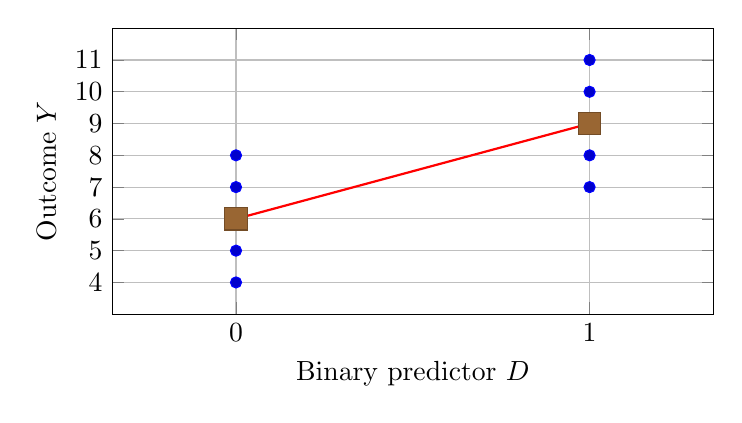
\begin{tikzpicture}
\begin{axis}[
    width=0.76\textwidth,
    height=0.43\textwidth,
    xlabel={Binary predictor \(D\)},
    ylabel={Outcome \(Y\)},
    xmin=-0.35, xmax=1.35,
    ymin=3, ymax=12,
    xtick={0,1},
    ytick={4,5,6,7,8,9,10,11},
    grid=major
]
\addplot+[only marks, mark=*] coordinates {
    (0,4) (0,5) (0,6) (0,7) (0,8)
    (1,7) (1,8) (1,9) (1,10) (1,11)
};
\addplot+[domain=0:1, samples=2, thick] {6 + 3*x};
\addplot+[only marks, mark=square*, mark size=4pt] coordinates {(0,6) (1,9)};
\end{axis}
\end{tikzpicture}
\caption{With a single binary predictor, OLS predicts each group's mean. The slope is therefore \(9-6=3\).}
\label{fig:binarymean}
\end{figure}

A base-R version of the same plot is:

\begin{lstlisting}
plot(jitter(dat_binary_ols$D, amount = 0.04), dat_binary_ols$Y,
     xaxt = "n",
     xlab = "Binary predictor D",
     ylab = "Outcome Y",
     main = "OLS with a Binary Predictor")
axis(1, at = c(0, 1), labels = c("D = 0", "D = 1"))

abline(fit_binary, lwd = 2)
points(c(0, 1),
       c(mean(dat_binary_ols$Y[dat_binary_ols$D == 0]),
         mean(dat_binary_ols$Y[dat_binary_ols$D == 1])),
       pch = 15, cex = 1.5)
\end{lstlisting}

This result is especially useful because many predictors in applied research are binary: treatment versus control, eligible versus ineligible, before versus after, male versus female, policy present versus absent, and so forth. The coefficient is a difference in conditional means for the two groups described by the model. Whether that difference should be interpreted \emph{causally} is a separate question and requires a causal design or causal assumptions.

\section{Regression Coefficients Are Instructions for Making Predictions}
\index{regression coefficient}\index{prediction}

Once a linear regression has been fitted, its coefficients provide a literal recipe for producing predicted values. For a simple regression,
\[
\widehat{Y}_i
=
\widehat{\beta}_0+
\widehat{\beta}_1X_i.
\]
R's \texttt{predict()} function is, in effect, applying this equation to the requested values of \(X\).

A useful empirical example is R's built-in \texttt{cars} dataset, which records automobile speeds (miles per hour) and stopping distances (feet). Fit

\begin{lstlisting}
fit_cars <- lm(dist ~ speed, data = cars)
summary(fit_cars)
coef(fit_cars)
\end{lstlisting}

The fitted coefficients are approximately
\[
\widehat{\beta}_0=-17.5791,
\qquad
\widehat{\beta}_1=3.9324.
\]
Thus the fitted prediction equation is
\[
\boxed{
\widehat{\text{dist}}
=
-17.5791 + 3.9324\,\text{speed}.
}
\]

There is nothing metaphorical about this equation. If speed is \(15\), R predicts
\[
-17.5791 + 3.9324(15)
\approx 41.407.
\]

\subsection{Predictions for the original training data}

If \texttt{newdata} is omitted, \texttt{predict()} returns fitted predictions for the observations used to estimate the model:

\begin{lstlisting}
# Predictions for the original training observations
train_predictions <- predict(fit_cars)

# The first several observed and predicted values
head(data.frame(
  speed = cars$speed,
  observed_dist = cars$dist,
  predicted_dist = train_predictions
))
\end{lstlisting}

These are the \(\widehat{Y}_i\)'s associated with the training sample. The residual for observation \(i\) is simply
\[
e_i=Y_i-\widehat{Y}_i.
\]
OLS chooses its coefficients to make the sum of the squared training residuals as small as possible.

\subsection{Predictions for new cases}

We can also supply a new test set containing predictor values that were not used as rows in the original regression call:

\begin{lstlisting}
new_cases <- data.frame(speed = c(10, 15, 20))

new_cases$predicted_dist <- predict(
  fit_cars,
  newdata = new_cases
)

new_cases
\end{lstlisting}

The predicted stopping distances are approximately
\[
21.745,\qquad 41.407,\qquad 61.069.
\]

We can verify that \texttt{predict()} is using the coefficients literally:

\begin{lstlisting}
b <- coef(fit_cars)

manual_predictions <-
  b[1] + b[2] * new_cases$speed

cbind(new_cases,
      manual_predictions = manual_predictions)
\end{lstlisting}

The manual calculations and \texttt{predict()} agree, up to numerical precision.

\begin{figure}[H]
\centering
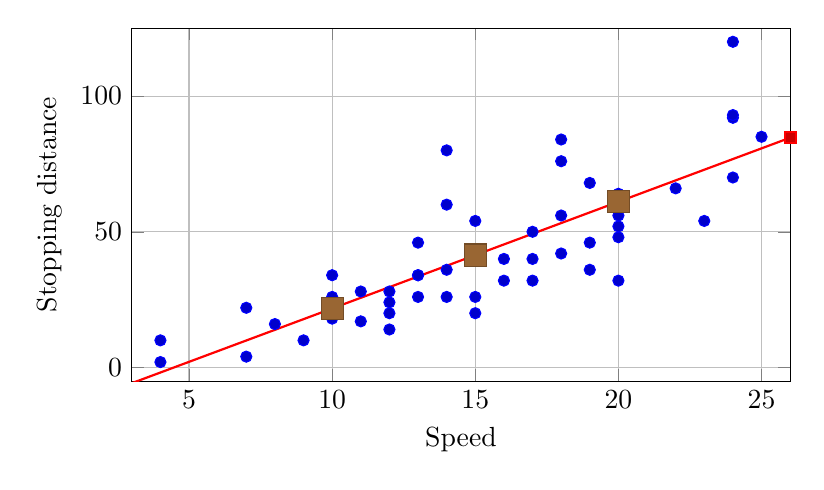
\begin{tikzpicture}
\begin{axis}[
    width=0.82\textwidth,
    height=0.50\textwidth,
    xlabel={Speed},
    ylabel={Stopping distance},
    xmin=3, xmax=26,
    ymin=-5, ymax=125,
    grid=major
]
\addplot+[only marks, mark=*] coordinates {
(4,2) (4,10) (7,4) (7,22) (8,16) (9,10)
(10,18) (10,26) (10,34) (11,17) (11,28)
(12,14) (12,20) (12,24) (12,28)
(13,26) (13,34) (13,34) (13,46)
(14,26) (14,36) (14,60) (14,80)
(15,20) (15,26) (15,54)
(16,32) (16,40)
(17,32) (17,40) (17,50)
(18,42) (18,56) (18,76) (18,84)
(19,36) (19,46) (19,68)
(20,32) (20,48) (20,52) (20,56) (20,64)
(22,66) (23,54) (24,70) (24,92) (24,93) (24,120) (25,85)
};
\addplot+[domain=3:26, samples=2, thick] {-17.57909489 + 3.93240876*x};
\addplot+[only marks, mark=square*, mark size=4pt] coordinates {
(10,21.74499) (15,41.40704) (20,61.06908)
};
\end{axis}
\end{tikzpicture}
\caption{The \texttt{cars} observations, the fitted OLS prediction line, and three predictions generated at speeds 10, 15, and 20.}
\label{fig:carspredict}
\end{figure}

The same visualization can be produced in base R:

\begin{lstlisting}
plot(cars$speed, cars$dist,
     xlab = "Speed",
     ylab = "Stopping distance",
     main = "Regression as a Prediction Rule")
abline(fit_cars, lwd = 2)

points(new_cases$speed,
       new_cases$predicted_dist,
       pch = 15, cex = 1.4)
\end{lstlisting}

The practical lesson is simple: a fitted linear regression is an equation, and \texttt{predict()} evaluates that equation for whichever predictor values we supply. The distinction between a \emph{training set} and a \emph{test set} concerns where those predictor values came from, not a different mathematical definition of the fitted regression.

\section{From a Coefficient Estimate to Statistical Uncertainty}

A regression coefficient such as \(\widehat{\beta}_1=3.9324\) is a point estimate: one number calculated from one sample. Statistical inference asks how much sampling uncertainty surrounds that estimate.

Two of the most familiar inferential quantities are the \(p\)-value and the confidence interval. They are related, but they answer different questions.

\subsection{What is a p-value?}
\index{p-value}

Suppose we test
\[
H_0:\beta_1=0.
\]
For ordinary OLS, R reports a test statistic of the form
\[
t=
\frac{\widehat{\beta}_1-0}
{\operatorname{SE}(\widehat{\beta}_1)}.
\]
The \(p\)-value asks how surprising a test statistic at least this incompatible with the null hypothesis would be \emph{if the null hypothesis were true and the assumptions used for the test were valid}.

A small \(p\)-value therefore says that the observed estimate is difficult to reconcile with the particular null hypothesis under the assumed statistical model. It does \emph{not} mean that the probability the null hypothesis is true is small. It also does not tell us whether an effect is substantively important.\footnote{\emph{Substantive importance} means importance in the real scientific, policy, practical, or decision context, rather than merely statistical detectability. An effect can be estimated very precisely and have a tiny \(p\)-value while still being too small to matter in practice.}

For the \texttt{cars} regression, the slope is about \(3.932\), its conventional standard error is about \(0.416\), and the resulting \(t\)-statistic is about \(9.46\). The conventional two-sided \(p\)-value is extremely small.

\subsection{What is a confidence interval for a regression coefficient?}
\index{confidence interval!coefficient}

A confidence interval gives a range of coefficient values produced by an inferential procedure. A \(95\%\) confidence procedure is designed so that, under repeated sampling from the assumed data-generating process, \(95\%\) of the intervals it constructs contain the target coefficient.

That repeated-sampling interpretation is important. After we have observed one sample, a conventional frequentist \(95\%\) confidence interval is not ordinarily interpreted as saying there is a \(95\%\) probability that the fixed coefficient lies inside this particular realized interval.

For an ordinary least-squares coefficient, the conventional \(95\%\) interval is
\[
\widehat{\beta}_j
\;\pm\;
 t_{0.975,\,df}
\operatorname{SE}(\widehat{\beta}_j),
\]
where the exact multiplier is a critical value from a \(t\) distribution with the appropriate residual degrees of freedom.

When the residual degrees of freedom are not tiny, that critical value is close to \(2\). Therefore a very useful approximation for a conventional \(95\%\) confidence interval for an OLS coefficient is
\[
\boxed{
\widehat{\beta}_j
\pm
2\operatorname{SE}(\widehat{\beta}_j).
}
\]

For the \texttt{cars} slope,
\[
3.9324 \pm 2(0.4155)
\]
gives approximately
\[
[3.10,4.76].
\]
The exact conventional \(t\)-based interval is approximately
\[
[3.097,4.768].
\]
So the two-standard-error rule is very close here.\footnote{For many maximum-likelihood regressions, including generalized linear models such as logit and Poisson, a Wald interval is similarly formed as approximately \(\widehat{\beta}\pm1.96\,\operatorname{SE}(\widehat{\beta})\) on the model's coefficient or link scale. If the quantity of interest is on a transformed scale, the interval endpoints can then be transformed appropriately---for example, exponentiating a logistic-regression coefficient interval to obtain an interval for an odds ratio, or using the inverse link for a fitted conditional mean. In small samples or difficult likelihood problems, simple Wald intervals may be poor approximations.}

In R:

\begin{lstlisting}
# Exact conventional confidence intervals for OLS coefficients
confint(fit_cars, level = 0.95)

# The familiar coefficient table
coef_table <- summary(fit_cars)$coefficients
coef_table

# Approximate 95% interval for the speed coefficient
b_speed <- coef_table["speed", "Estimate"]
se_speed <- coef_table["speed", "Std. Error"]

b_speed + c(-1, 1) * 2 * se_speed
\end{lstlisting}

\subsection{A tiny p-value does not imply a tight confidence interval}

It is easy to think that an extremely small \(p\)-value must imply a very narrow confidence interval. It does not.

The width of the approximate \(95\%\) confidence interval is controlled by the standard error:
\[
\text{width}\approx 4\operatorname{SE}(\widehat{\beta}).
\]
The \(p\)-value for testing \(\beta=0\), by contrast, is driven largely by the ratio
\[
\frac{|\widehat{\beta}|}{\operatorname{SE}(\widehat{\beta})}.
\]

For example, consider two hypothetical estimates:
\[
\widehat{\beta}_A=100,
\qquad
\operatorname{SE}(\widehat{\beta}_A)=20,
\]
and
\[
\widehat{\beta}_B=0.05,
\qquad
\operatorname{SE}(\widehat{\beta}_B)=0.01.
\]
Both have a test statistic of magnitude \(5\), and therefore both produce very small \(p\)-values when testing against zero. Yet the approximate \(95\%\) confidence intervals are
\[
[60,140]
\]
and
\[
[0.03,0.07],
\]
respectively. One interval is numerically very wide and the other very narrow. The \(p\)-value is primarily telling us how far the estimate lies from the null in standard-error units; it is not itself a measure of the absolute precision or width of the confidence interval.

\section{When Does a Confidence Interval Achieve Its Nominal Coverage?}
\index{coverage}

The phrase ``\(95\%\) confidence interval'' is a promise about a procedure: under the conditions for which that procedure was derived, repeated applications of it should cover the target parameter about \(95\%\) of the time.

The phrase \emph{under the conditions} is essential. A confidence interval cannot be expected to achieve its nominal coverage simply because software labels the output a ``95\% confidence interval.'' The assumptions required by the inferential procedure must be sufficiently appropriate for the target being estimated.

For the conventional textbook OLS standard errors and confidence intervals, proper specification typically requires several things. Most importantly, the conditional mean must have the form the regression claims it has:
\[
\E[Y\mid X]
=
X\beta.
\]
In a one-predictor model, this means that the true conditional mean is adequately described by the specified line or by whatever transformations and interactions have been explicitly included. If the true conditional mean bends sharply but the model insists on a straight line, the model is misspecified as a model of that conditional mean.

The conventional textbook variance formula also assumes a suitable error structure.\footnote{By \emph{error structure}, we mean features of the unexplained variation around the conditional mean that matter for uncertainty calculations---especially its variance and any dependence across observations. For example, errors may have different variances in different parts of the predictor space, or observations from the same school, household, firm, or time series may have correlated errors.} In its simplest form, this includes constant conditional error variance (homoskedasticity) and an independence structure appropriate to the sampling process. Exact small-sample \(t\) inference additionally relies on normal-error assumptions; large-sample approximations can relax normality substantially. Other data structures---for example clustered, serially correlated, or heteroskedastic observations---require uncertainty procedures designed for those structures.

Some assumption failures can be handled with robust methods.\footnote{\emph{Robust} does not mean assumption-free. A robust procedure is designed to remain valid when a particular assumption is relaxed or violated. Heteroskedasticity-robust standard errors, for example, relax the constant-variance assumption, but they still require other conditions for their large-sample justification.} Heteroskedasticity-robust standard errors, for example, are designed precisely so that heteroskedasticity need not invalidate large-sample coefficient inference under appropriate conditions. The general principle is therefore not that every statistical model must be literally perfect. It is that the assumptions required by the particular confidence procedure, for the particular estimand\footnote{An \emph{estimand} is the population quantity an analysis is trying to learn about---for example, a regression slope, a conditional mean at a specified value of \(X\), or an average treatment effect. The \emph{estimator} is the rule used to estimate that quantity from data; the \emph{estimate} is the numerical result obtained in one sample.} we claim to be covering, must be adequate. If they are not, the nominal \(95\%\) label does not guarantee \(95\%\) coverage.

\subsection{Why ``properly specified'' is hard to know in real research}

In many real-world applications, analysts do not know the true conditional expectation function. That is one reason they are using regression in the first place.

Suppose we are predicting wages from education, experience, occupation, region, and other variables. Is the effect of experience linear? Does it flatten with age? Does education interact with occupation? Are relevant predictors missing? Does error variance differ across groups? Are observations independent, or are people nested inside common labor markets? There is rarely a known mathematical law that settles these questions.

Diagnostics can help us find evidence that a specification is inadequate. Residual plots may reveal curvature or heteroskedasticity. Subject-matter knowledge may suggest important interactions. Flexible models can be compared with restrictive ones. But failure to detect a problem is not proof that the model is correctly specified. Many different data-generating mechanisms can look similar in one finite sample.

Natural sciences sometimes provide unusually strong structural guidance because the relevant relationship may be governed, under known conditions, by a physical formula. For example, elementary kinematics tells us that under constant acceleration,
\[
s(t)=s_0+v_0t+\frac{1}{2}at^2.
\]
That knowledge gives the analyst unusually strong guidance about functional form. Even then, measurements can contain error and real systems can violate idealized conditions. But in many social, behavioral, economic, policy, and biological applications, there is no comparably exact known formula for the conditional mean.

For that reason, analysts should treat confidence-interval coverage and \(p\)-value calibration\footnote{A testing procedure is well calibrated when its stated error rates match its actual repeated-sampling behavior under the conditions being claimed. For example, under a true null hypothesis, a properly calibrated 5\% test rejects about 5\% of the time across repeated samples; equivalently, valid null \(p\)-values fall below 0.05 about 5\% of the time.} as properties that depend on assumptions, not as automatic features of regression output. We can often make those assumptions more plausible, and we can use robust procedures for some known problems, but we usually cannot prove that our specification is the true one.

This is the distinction introduced in Chapter~\ref{chap:intro}: optimization of the training objective is built into the fitting algorithm. Correct inferential calibration is not.

\section{Mean Squared Error: Measuring Prediction Error}
\index{mean squared error}

Before introducing \(R^2\), it is helpful to start with a direct measure of prediction performance.

For observed outcomes \(Y_i\) and predictions \(\widehat{Y}_i\), define prediction mean squared error as
\[
\MSE
=
\frac{1}{n}
\sum_{i=1}^{n}
(Y_i-\widehat{Y}_i)^2.
\]
Each prediction error is squared, the squared errors are added, and the total is divided by the number of observations. Smaller MSE means that, under squared-error loss, predictions are closer to the observed outcomes on average.

Here ``MSE'' means the average squared \emph{prediction error} using divisor \(n\). This is the quantity useful for the \(R^2\) interpretation below. It should not be confused with the residual mean square sometimes used to estimate \(\sigma^2\), which uses residual degrees of freedom rather than \(n\).

\section{The Zero-Predictor Benchmark: Predict Everyone With the Mean}
\index{mean-only model}

What would linear regression do if we gave it no predictors at all?

With only an intercept,
\[
Y_i=\beta_0+\varepsilon_i,
\]
OLS chooses
\[
\widehat{\beta}_0=\overline{Y}.
\]
It therefore makes exactly the same prediction for every observation:
\[
\widehat{Y}_i=\overline{Y}
\qquad\text{for every }i.
\]

This is not arbitrary. Among all possible single constant predictions, the sample mean is the number that minimizes the sum of squared errors. If we refuse to give the regression any information about how observations differ from one another, predicting the overall mean is the best squared-error prediction it can make.

That intercept-only model provides a natural baseline. For OLS with an intercept, adding predictors cannot increase the training-sample sum of squared errors when we evaluate the same observations. The expanded model can always reproduce the old fit by assigning zero coefficients to predictors that do not help, and it may reduce squared error if the added predictors contain useful predictive information.

This claim is specifically about \emph{training-sample} OLS. On a genuinely new test set, an overfit or unstable model can predict worse than the simple mean benchmark.

\section{What \(R^2\) Measures}
\index{R-squared@$R^2$}

Now suppose the mean-only model has prediction MSE equal to \(50\). We add one predictor, fit OLS, and the model's training MSE falls to \(10\).

The predictor has removed
\[
50-10=40
\]
units of squared prediction error from an original \(50\). The fraction removed is
\[
\frac{50-10}{50}=0.80.
\]
So \(80\%\) of the squared error made by the zero-predictor, mean-only model has disappeared.

That is essentially what \(R^2\) measures. For an OLS regression containing an intercept,
\[
R^2
=
1-
\frac{\sum_i(Y_i-\widehat{Y}_i)^2}
{\sum_i(Y_i-\overline{Y})^2}.
\]
If we divide both numerator and denominator by \(n\), the same formula becomes
\[
\boxed{
R^2
=
1-
\frac{\MSE_{\text{model}}}
{\MSE_{\text{mean-only}}}.
}
\]
Thus \(R^2\) is the fraction of the mean-only model's training squared prediction error that disappears when the predictors are used.

If \(R^2=0.80\), the regression has removed \(80\%\) of the squared prediction error associated with predicting everyone by the overall mean. If \(R^2=0\), the fitted predictors have not improved on the mean-only benchmark at all.

If
\[
R^2=1,
\]
then
\[
\sum_i(Y_i-\widehat{Y}_i)^2=0.
\]
Every training observation is predicted perfectly:
\[
\widehat{Y}_i=Y_i
\qquad\text{for every }i.
\]
This is the best possible training-sample squared-error performance. There is no residual prediction error left to remove.

\subsection{An empirical example using \texttt{cars}}

Return to the regression
\[
\text{dist}_i
=
\beta_0+\beta_1\text{speed}_i+\varepsilon_i.
\]
For the \texttt{cars} data, the mean-only prediction MSE is approximately
\[
650.78.
\]
After speed is added as a predictor, the training prediction MSE is approximately
\[
227.07.
\]
Therefore
\[
R^2
=
1-\frac{227.07}{650.78}
\approx 0.651.
\]

About \(65\%\) of the squared prediction error made by the mean-only model disappears when speed is used to predict stopping distance.

The base-R calculations are:

\begin{lstlisting}
fit_cars <- lm(dist ~ speed, data = cars)

# R-squared reported by lm()
summary(fit_cars)$r.squared

# Reconstruct R-squared from prediction MSE
mse_mean_only <- mean(
  (cars$dist - mean(cars$dist))^2
)

mse_model <- mean(
  (cars$dist - predict(fit_cars))^2
)

1 - mse_model / mse_mean_only
\end{lstlisting}

Both calculations return approximately \(0.6511\).

\section{Why Adding Predictors Cannot Lower Training \(R^2\)}

Suppose we start with
\[
\widehat{Y}
=
\widehat{\beta}_0+
\widehat{\beta}_1X_1
\]
and then add another predictor:
\[
\widehat{Y}
=
\widehat{\beta}_0+
\widehat{\beta}_1X_1+
\widehat{\beta}_2X_2.
\]

The second model contains the first model as a special case. If \(X_2\) is useless, OLS is allowed to choose \(\widehat{\beta}_2=0\), in which case it can reproduce the fit of the smaller model. If \(X_2\) is useful for reducing training squared error, OLS can choose a nonzero coefficient and improve the fit.

Therefore, on the same training observations,
\[
\text{SSE}_{\text{larger model}}
\leq
\text{SSE}_{\text{smaller model}},
\]
and hence
\[
R^2_{\text{larger model}}
\geq
R^2_{\text{smaller model}}.
\]
Training \(R^2\) can stay the same or rise when predictors are added; it cannot fall.

This is also why a larger training \(R^2\) does not automatically mean that a model is better for predicting new cases. A model can use extra flexibility to fit noise in the training data. Test-set prediction must be evaluated on data that were not used to choose the coefficients.

\subsection{Use ordinary \(R^2\) in this book}

R also reports an \emph{adjusted} \(R^2\), which applies a penalty related to the number of predictors. Adjusted \(R^2\) answers a different model-comparison question and can decrease when predictors are added.

For our purposes, \textbf{use ordinary \(R^2\), not adjusted \(R^2\)}. Ordinary \(R^2\) has the clean interpretation developed here: it is the fraction of the mean-only model's training squared prediction error removed by the fitted predictors. When an exercise asks for \(R^2\), do not substitute adjusted \(R^2\).

\section{Putting the Pieces Together}

Several facts that can initially seem unrelated are really different views of the same prediction machine.

With a binary predictor, OLS predicts one mean for the zero group and one mean for the one group; the coefficient is therefore the difference between those two means. With a continuous predictor, the fitted coefficients define an equation, and \texttt{predict()} evaluates that equation for training observations or new cases. A coefficient's standard error describes sampling uncertainty, and conventional \(p\)-values and confidence intervals use that uncertainty under a set of statistical assumptions. Those inferential guarantees are not automatic when the assumptions underlying the procedure are badly wrong. Finally, \(R^2\) compares the model's training squared prediction error with the error from the simplest possible OLS benchmark: predicting every observation with the sample mean.

Seen this way, coefficients, predictions, residuals, uncertainty, MSE, and \(R^2\) are not separate pieces of statistical vocabulary. They are connected components of the same regression framework.


\chapter{Uncertainty Around Predictions and Interpreting Multiple Regression}
\index{prediction interval}\index{confidence interval!predicted mean}\index{multiple regression}
\label{chap:intervals_multiple}

Regression gives us point predictions, but point predictions are only part of the story. We also need to understand uncertainty. The terminology is potentially confusing because regression uses similar language for several \emph{different} kinds of uncertainty.

This chapter has two goals. First, it distinguishes three objects that students must keep separate:

\begin{enumerate}
    \item a confidence interval for a regression \emph{coefficient};
    \item a confidence interval for a \emph{predicted conditional mean}---that is, uncertainty about where the regression line is;
    \item a prediction interval for a \emph{new observed outcome}---that is, uncertainty about where an individual data point might lie.
\end{enumerate}

Second, the chapter explains how to interpret coefficients once a regression contains more than one predictor. The phrase ``holding other variables fixed'' will become concrete: it describes a comparison between predictions that differ in one predictor while the other predictors are kept at the same values.

\section{Three Different Uncertainty Questions}
\index{confidence interval}\index{prediction interval}

Consider the simple linear regression
\[
Y_i=\beta_0+\beta_1X_i+\varepsilon_i.
\]

After fitting the model, we have a line
\[
\widehat{Y}_i=\widehat{\beta}_0+\widehat{\beta}_1X_i.
\]

There are at least three distinct uncertainty questions we might ask.

\begin{center}
\fbox{
\parbox{0.92\textwidth}{
\textbf{Do not say simply ``the confidence interval'' without specifying what the interval is for.}

\vspace{0.5em}

\textbf{1. Confidence interval for a coefficient}

Target: an unknown regression coefficient such as \(\beta_1\).

Question: \emph{How uncertain are we about the slope parameter?}

Typical R command:
\[
\texttt{confint(fit)}
\]

\vspace{0.75em}

\textbf{2. Confidence interval for a predicted mean}

Target: the conditional mean \(E[Y\mid X=x]\).

Question: \emph{Where is the regression line likely to be at this value of \(X\)?}

Typical R command:
\[
\texttt{predict(fit, newdata = ..., interval = "confidence")}
\]

\vspace{0.75em}

\textbf{3. Prediction interval for a new outcome}

Target: a new individual value \(Y_{\text{new}}\) at \(X=x\).

Question: \emph{Where might an actual new data point lie?}

Typical R command:
\[
\texttt{predict(fit, newdata = ..., interval = "prediction")}
\]

\vspace{0.75em}

\textbf{These are not three names for the same thing. They are three different inferential targets.}
}}
\end{center}

The nomenclature is especially unfortunate because the phrase \emph{confidence interval} is used in both the first and second cases. A ``95\% confidence interval'' might refer to uncertainty about a coefficient, or it might refer to uncertainty about a predicted mean. Context matters.

A good habit is therefore to use the full phrase:

\begin{itemize}
    \item ``95\% confidence interval for the slope coefficient'';
    \item ``95\% confidence interval for the fitted mean at \(X=15\)'';
    \item ``95\% prediction interval for a new observation at \(X=15\)''.
\end{itemize}

If you always name the target, the ambiguity mostly disappears.

\section{Confidence Intervals for Regression Coefficients}
\index{confidence interval!coefficient}

Suppose we estimate
\[
Y_i=\beta_0+\beta_1X_i+\varepsilon_i
\]
and obtain the fitted slope \(\widehat{\beta}_1\).

The coefficient \(\widehat{\beta}_1\) is a point estimate. A confidence interval for \(\beta_1\) describes uncertainty about the underlying regression coefficient.

For ordinary least squares under the usual linear-model assumptions, a \(100(1-\alpha)\%\) confidence interval for coefficient \(\beta_j\) has the form
\[
\widehat{\beta}_j
\pm
t_{1-\alpha/2,\;df}
\operatorname{SE}(\widehat{\beta}_j).
\]

For a 95\% interval, the critical value is often close to 2 in moderate or large samples, so a useful approximation is
\[
\widehat{\beta}_j
\pm
2\operatorname{SE}(\widehat{\beta}_j).
\]

This is the kind of confidence interval discussed when we examine uncertainty in the coefficients printed by \texttt{summary(lm(...))}.

For example:

\begin{lstlisting}
fit <- lm(dist ~ speed, data = cars)

summary(fit)
confint(fit)
\end{lstlisting}

The call to \texttt{confint(fit)} returns confidence intervals for the intercept and the slope. These intervals are about \(\beta_0\) and \(\beta_1\). They are \emph{not} intervals telling us where future stopping distances will lie.

A simple coefficient-interval visualization can be made with base R:

\begin{lstlisting}
fit <- lm(dist ~ speed, data = cars)

slope <- coef(fit)["speed"]
slope_ci <- confint(fit)["speed", ]

plot(
  1, slope,
  xlim = c(0.5, 1.5),
  ylim = range(c(0, slope_ci)),
  xaxt = "n",
  xlab = "",
  ylab = "Slope coefficient for speed",
  pch = 19
)

segments(
  x0 = 1,
  y0 = slope_ci[1],
  x1 = 1,
  y1 = slope_ci[2],
  lwd = 3
)

points(1, slope, pch = 19)
axis(1, at = 1, labels = "speed")
abline(h = 0, lty = 3)
\end{lstlisting}

This graph displays uncertainty about \emph{one coefficient}. It should not be confused with the bands that we will soon draw around the fitted regression line.

\section{Two Different Intervals for Predictions}

Now suppose our question is not about the slope coefficient itself. Instead, suppose we want to use the fitted regression to make a prediction at a particular value \(X=x_0\).

The fitted value is
\[
\widehat{Y}(x_0)
=
\widehat{\beta}_0+\widehat{\beta}_1x_0.
\]

There are now \emph{two different uncertainty questions} we might ask.

\subsection{Confidence interval for the predicted mean: where is the regression line?}
\index{confidence interval!predicted mean}

The first question is:

\begin{quote}
At \(X=x_0\), where is the true conditional mean \(E[Y\mid X=x_0]\) likely to be?
\end{quote}

This is uncertainty about the \emph{regression function itself}. We estimated the line from a finite sample, so another random sample would generally produce a somewhat different line. The fitted line therefore has sampling uncertainty.

In R, for ordinary linear regression:

\begin{lstlisting}
fit <- lm(dist ~ speed, data = cars)

predict(
  fit,
  newdata = data.frame(speed = 15),
  interval = "confidence",
  level = 0.95
)
\end{lstlisting}

The output contains three columns:

\begin{itemize}
    \item \texttt{fit}: the point prediction;
    \item \texttt{lwr}: the lower end of the confidence interval;
    \item \texttt{upr}: the upper end of the confidence interval.
\end{itemize}

The interval is about the mean stopping distance predicted by the regression at speed \(15\). It is an interval for the location of the regression line at \(X=15\).

It is \emph{not} intended to contain 95\% of individual cars' stopping distances.

\subsection{Prediction interval: where might a new data point lie?}
\index{prediction interval}

The second question is different:

\begin{quote}
If we observe one new unit with \(X=x_0\), where might its actual \(Y\) value lie?
\end{quote}

Even if we knew the regression line perfectly, individual observations would still scatter above and below that line. A prediction interval has to account for both:

\begin{enumerate}
    \item uncertainty about where the regression line is; and
    \item the ordinary unit-to-unit variation of observations around that line.
\end{enumerate}

In R:

\begin{lstlisting}
predict(
  fit,
  newdata = data.frame(speed = 15),
  interval = "prediction",
  level = 0.95
)
\end{lstlisting}

This interval is about a \emph{new observed stopping distance}, not merely about the conditional mean stopping distance.

That is why a prediction interval is ordinarily wider than the corresponding confidence interval for the fitted mean.

\subsection{Why the prediction interval is wider}

For simple linear regression, the standard error used for a confidence interval around the fitted mean at \(x_0\) is
\[
s
\sqrt{
\frac{1}{n}
+
\frac{(x_0-\bar{x})^2}
{\sum_{i=1}^{n}(x_i-\bar{x})^2}
}.
\]

For a prediction interval for a new observation, the corresponding quantity is
\[
s
\sqrt{
1+
\frac{1}{n}
+
\frac{(x_0-\bar{x})^2}
{\sum_{i=1}^{n}(x_i-\bar{x})^2}
}.
\]

The prediction interval contains an extra \(1\) under the square root.

Conceptually, that extra term represents the fact that the new observation itself can fall above or below the conditional mean. The confidence interval for the fitted mean asks only where the regression line is. The prediction interval asks where a noisy new data point might appear.

\begin{center}
\fbox{
\parbox{0.88\textwidth}{
\centering
\textbf{Confidence interval for a predicted mean: uncertainty about the line.}

\vspace{0.4em}

\textbf{Prediction interval: uncertainty about a new data point.}

\vspace{0.4em}

\textbf{Prediction intervals are therefore ordinarily wider.}
}}
\end{center}

\section{Visualizing the Two Prediction Intervals}

The following schematic picture shows the distinction. The narrow inner band represents uncertainty about the conditional mean. The wider outer band represents uncertainty about where a new observation might lie.

\begin{figure}[H]
\centering
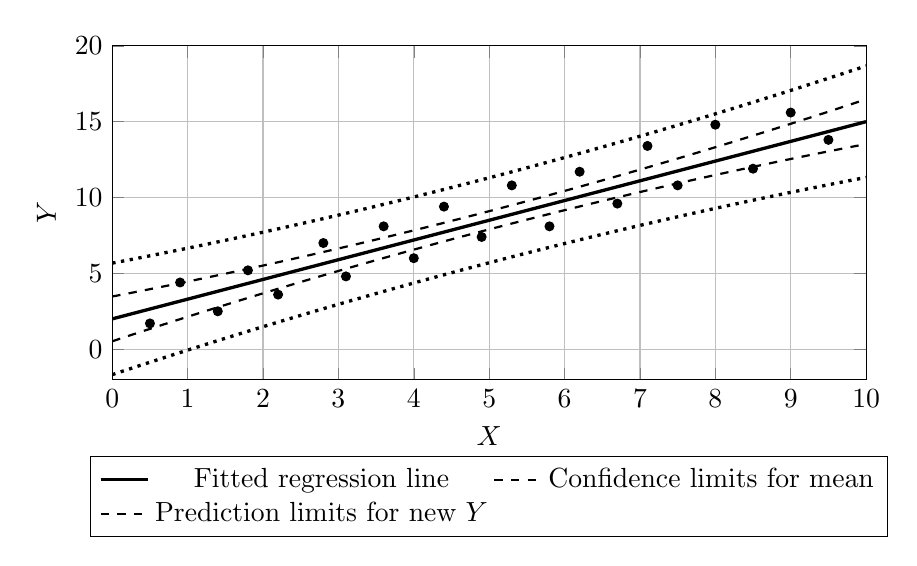
\begin{tikzpicture}
\begin{axis}[
    width=0.92\textwidth,
    height=0.48\textwidth,
    xlabel={$X$},
    ylabel={$Y$},
    xmin=0, xmax=10,
    ymin=-2, ymax=20,
    legend style={at={(0.5,-0.23)},anchor=north,legend columns=2},
    grid=major
]

\addplot[
    domain=0:10,
    samples=100,
    very thick
]
{2 + 1.3*x};
\addlegendentry{Fitted regression line}

\addplot[
    domain=0:10,
    samples=100,
    dashed,
    thick
]
{2 + 1.3*x + 0.6 + 0.035*(x-5)^2};
\addlegendentry{Confidence limits for mean}

\addplot[
    domain=0:10,
    samples=100,
    dashed,
    thick
]
{2 + 1.3*x - 0.6 - 0.035*(x-5)^2};

\addplot[
    domain=0:10,
    samples=100,
    dotted,
    very thick
]
{2 + 1.3*x + 2.8 + 0.035*(x-5)^2};
\addlegendentry{Prediction limits for new $Y$}

\addplot[
    domain=0:10,
    samples=100,
    dotted,
    very thick
]
{2 + 1.3*x - 2.8 - 0.035*(x-5)^2};

\addplot[
    only marks,
    mark=*,
    mark size=1.6pt
]
coordinates {
(0.5,1.7)
(0.9,4.4)
(1.4,2.5)
(1.8,5.2)
(2.2,3.6)
(2.8,7.0)
(3.1,4.8)
(3.6,8.1)
(4.0,6.0)
(4.4,9.4)
(4.9,7.4)
(5.3,10.8)
(5.8,8.1)
(6.2,11.7)
(6.7,9.6)
(7.1,13.4)
(7.5,10.8)
(8.0,14.8)
(8.5,11.9)
(9.0,15.6)
(9.5,13.8)
};

\end{axis}
\end{tikzpicture}
\caption{The confidence band for the conditional mean is narrower than the prediction band for a new observation. The figure is schematic: its purpose is to distinguish the targets.}
\label{fig:ci_pi_schematic}
\end{figure}

A useful way to read Figure~\ref{fig:ci_pi_schematic} is to imagine choosing a single vertical slice at \(X=5\).

At that \(X\)-value:

\begin{itemize}
    \item the fitted line gives one point prediction;
    \item the two dashed boundaries describe uncertainty about the height of the true regression line;
    \item the two dotted boundaries describe a much wider range in which a new individual observation might plausibly fall.
\end{itemize}

The width of the confidence band is typically smallest near the center of the observed \(X\)-values and grows toward the edges. We have more information about the regression function where the data are concentrated. The prediction interval shows the same pattern, but remains wider because it must also incorporate residual variation.

\section{Base R Example: Plotting Both Bands with the \texttt{cars} Data}

The built-in R dataset \texttt{cars} contains automobile speeds (miles per hour) and stopping distances (feet). We can fit
\[
\text{distance}
=
\beta_0+\beta_1\text{speed}+\varepsilon
\]
and then ask R for both kinds of prediction intervals.

\begin{lstlisting}
# Fit the regression
fit <- lm(dist ~ speed, data = cars)

# Create a dense grid of speed values for smooth interval bands
speed_grid <- data.frame(
  speed = seq(
    from = min(cars$speed),
    to = max(cars$speed),
    length.out = 200
  )
)

# Confidence interval for the conditional mean
conf_band <- predict(
  fit,
  newdata = speed_grid,
  interval = "confidence",
  level = 0.95
)

# Prediction interval for a new observation
pred_band <- predict(
  fit,
  newdata = speed_grid,
  interval = "prediction",
  level = 0.95
)

# Plot the observed data
plot(
  cars$speed,
  cars$dist,
  xlab = "Speed",
  ylab = "Stopping distance",
  main = "Confidence and Prediction Intervals"
)

# Fitted regression line
lines(
  speed_grid$speed,
  conf_band[, "fit"],
  lwd = 3
)

# Confidence limits for the conditional mean
lines(
  speed_grid$speed,
  conf_band[, "lwr"],
  lty = 2,
  lwd = 2
)

lines(
  speed_grid$speed,
  conf_band[, "upr"],
  lty = 2,
  lwd = 2
)

# Prediction limits for a new observation
lines(
  speed_grid$speed,
  pred_band[, "lwr"],
  lty = 3,
  lwd = 2
)

lines(
  speed_grid$speed,
  pred_band[, "upr"],
  lty = 3,
  lwd = 2
)

legend(
  "topleft",
  legend = c(
    "Regression line",
    "Confidence interval for mean",
    "Prediction interval for new observation"
  ),
  lty = c(1, 2, 3),
  lwd = c(3, 2, 2),
  bty = "n"
)
\end{lstlisting}

The important visual fact is not merely that one pair of lines is wider than the other. It is \emph{why}.

The inner confidence band answers:
\[
\text{Where is }E[Y\mid X=x]\text{?}
\]

The outer prediction band answers:
\[
\text{Where might }Y_{\text{new}}\text{ be at }X=x\text{?}
\]

Those are different questions.

\section{Seeing the Three Targets Side by Side in R}

The distinction becomes especially clear if we make all three requests explicitly.

\begin{lstlisting}
fit <- lm(dist ~ speed, data = cars)

# 1. Confidence intervals for regression coefficients
confint(fit)

# 2. Confidence interval for the predicted mean at speed = 15
predict(
  fit,
  newdata = data.frame(speed = 15),
  interval = "confidence"
)

# 3. Prediction interval for one new observation at speed = 15
predict(
  fit,
  newdata = data.frame(speed = 15),
  interval = "prediction"
)
\end{lstlisting}

These commands return fundamentally different objects.

The first concerns \(\beta_0\) and \(\beta_1\).

The second concerns
\[
E[Y\mid X=15].
\]

The third concerns
\[
Y_{\text{new}}\mid X=15.
\]

One way to prevent confusion is to ask yourself, before requesting an interval:

\begin{quote}
\textbf{What is the unknown quantity I want this interval to cover?}
\end{quote}

If the answer is ``the slope,'' you want a coefficient confidence interval.

If the answer is ``the location of the regression line at this \(X\),'' you want a confidence interval for the fitted mean.

If the answer is ``the outcome of one new unit,'' you want a prediction interval.

\section{The Same Point Prediction Sits at the Center of Both Prediction Intervals}

Notice that the confidence interval for the conditional mean and the prediction interval for a new observation are centered on the same fitted value.

For example:

\begin{lstlisting}
fit <- lm(dist ~ speed, data = cars)

b <- coef(fit)

# Calculate the prediction literally from the coefficients
manual_prediction <- b[1] + b[2] * 15
manual_prediction

# Ask predict() for the point prediction
predict(
  fit,
  newdata = data.frame(speed = 15)
)
\end{lstlisting}

The two point predictions are the same, up to numerical precision.

The intervals differ not because R is using a different regression line, but because R is answering different uncertainty questions around that same fitted value.

This is an important conceptual pattern:

\[
\text{same point prediction}
\quad+\quad
\text{different target}
\quad=\quad
\text{different interval}.
\]

\section{Coverage Requires Assumptions}

The words ``95\% confidence interval'' and ``95\% prediction interval'' refer to repeated-sampling coverage properties under a statistical model.

For the standard finite-sample OLS intervals taught in an introductory course, the assumptions include an appropriate linear conditional-mean specification and assumptions about the disturbances used by the standard formulas. Exact textbook \(t\)-intervals additionally rely on normality of the errors. Conventional prediction intervals also ordinarily rely on constant conditional error variance when the usual homoskedastic formula is used.

If these assumptions fail, the nominal coverage can fail as well.

This does not mean that every departure from a textbook assumption destroys an analysis. Robust standard errors, alternative variance models, transformations, flexible regression functions, bootstrap procedures, and other methods can address particular problems. But the label ``95\%'' does not, by itself, guarantee correct coverage merely because the interval was produced by \texttt{confint()} or \texttt{predict()}.

The interval inherits its interpretation from the assumptions and procedure used to construct it.

That warning applies to all three interval concepts in this chapter.

\section{From Simple to Multiple Regression}
\index{multiple regression}\index{holding other variables fixed}

We now turn to a different foundational issue: what happens to coefficient interpretation when a regression contains more than one predictor?

Begin with
\[
Y_i
=
\beta_0+\beta_1X_i+\varepsilon_i.
\]

Here, \(\beta_1\) describes how the fitted value of \(Y\) changes as \(X\) changes.

Now add another predictor \(Z\):
\[
Y_i
=
\beta_0+\beta_1X_i+\beta_2Z_i+\varepsilon_i.
\]

The fitted prediction is
\[
\widehat{Y}
=
\widehat{\beta}_0
+
\widehat{\beta}_1X
+
\widehat{\beta}_2Z.
\]

What does \(\widehat{\beta}_1\) mean now?

Compare two otherwise identical prediction inputs:

\[
(X,Z)
\]
and
\[
(X+1,Z).
\]

The first prediction is
\[
\widehat{Y}(X,Z)
=
\widehat{\beta}_0
+
\widehat{\beta}_1X
+
\widehat{\beta}_2Z.
\]

The second is
\[
\widehat{Y}(X+1,Z)
=
\widehat{\beta}_0
+
\widehat{\beta}_1(X+1)
+
\widehat{\beta}_2Z.
\]

Subtracting,
\[
\widehat{Y}(X+1,Z)
-
\widehat{Y}(X,Z)
=
\widehat{\beta}_1.
\]

This is what ``holding \(Z\) fixed'' means mathematically.

\begin{center}
\fbox{
\parbox{0.88\textwidth}{
\centering
In a multiple regression, the coefficient on \(X\) describes how the model's prediction changes when \(X\) changes by one unit \textbf{while the other included predictors are kept at the same values}.
}}
\end{center}

This is a statement about the fitted prediction function. It does not require us literally to reach into the world and physically freeze all other variables.

\section{A Binary Predictor in Multiple Regression}

Suppose \(D\) is binary:
\[
D=
\begin{cases}
0\\
1.
\end{cases}
\]

Consider
\[
Y_i
=
\beta_0+\beta_1X_i+\beta_2D_i+\varepsilon_i.
\]

For \(D=0\),
\[
\widehat{Y}
=
\widehat{\beta}_0+\widehat{\beta}_1X.
\]

For \(D=1\),
\[
\widehat{Y}
=
\widehat{\beta}_0+\widehat{\beta}_1X+\widehat{\beta}_2.
\]

At the same value of \(X\), the difference is
\[
\widehat{\beta}_2.
\]

Thus \(\widehat{\beta}_2\) is the fitted difference between the two groups \emph{at the same value of \(X\)}.

Because there is no interaction between \(X\) and \(D\), the model assumes that this difference is constant for all values of \(X\). Graphically, the two fitted regression lines are parallel.

\begin{figure}[H]
\centering
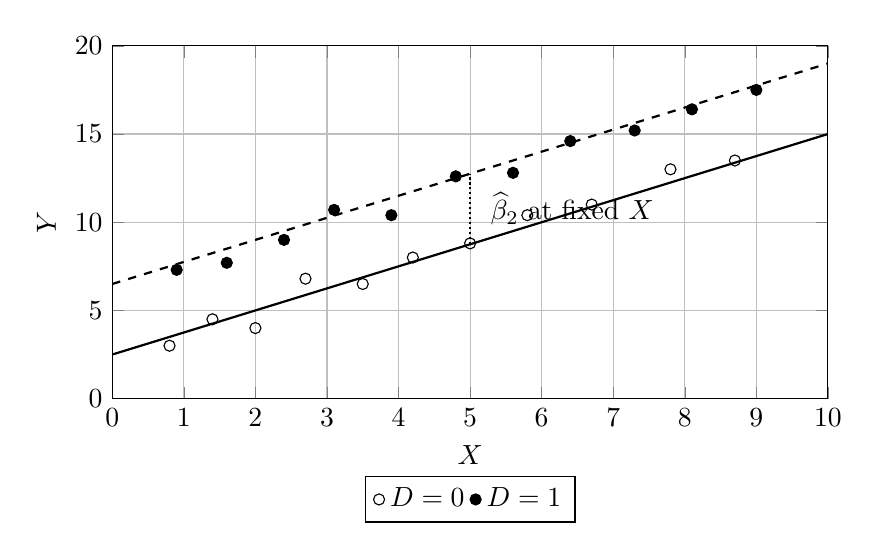
\begin{tikzpicture}
\begin{axis}[
    width=0.88\textwidth,
    height=0.5\textwidth,
    xlabel={$X$},
    ylabel={$Y$},
    xmin=0, xmax=10,
    ymin=0, ymax=20,
    legend style={at={(0.5,-0.22)},anchor=north,legend columns=2},
    grid=major
]

\addplot[
    only marks,
    mark=o,
    mark size=2pt
]
coordinates {
(0.8,3.0)
(1.4,4.5)
(2.0,4.0)
(2.7,6.8)
(3.5,6.5)
(4.2,8.0)
(5.0,8.8)
(5.8,10.4)
(6.7,11.0)
(7.8,13.0)
(8.7,13.5)
};
\addlegendentry{$D=0$}

\addplot[
    only marks,
    mark=*,
    mark size=2pt
]
coordinates {
(0.9,7.3)
(1.6,7.7)
(2.4,9.0)
(3.1,10.7)
(3.9,10.4)
(4.8,12.6)
(5.6,12.8)
(6.4,14.6)
(7.3,15.2)
(8.1,16.4)
(9.0,17.5)
};
\addlegendentry{$D=1$}

\addplot[
    domain=0:10,
    samples=2,
    thick
]
{2.5 + 1.25*x};

\addplot[
    domain=0:10,
    samples=2,
    thick,
    dashed
]
{6.5 + 1.25*x};

\draw[densely dotted, thick]
(axis cs:5,8.75) -- (axis cs:5,12.75);

\node[
    anchor=west
] at (axis cs:5.15,10.75)
{\(\widehat{\beta}_2\) at fixed \(X\)};

\end{axis}
\end{tikzpicture}
\caption{With no interaction, a binary predictor shifts the fitted line vertically while the slope on \(X\) remains the same. The coefficient on \(D\) is the vertical difference between predictions at the same \(X\).}
\label{fig:multiple_parallel}
\end{figure}

\section{An Empirical Example with \texttt{mtcars}}

The built-in \texttt{mtcars} data provide a useful example.

Let:

\begin{itemize}
    \item \texttt{mpg} be miles per gallon;
    \item \texttt{am} equal 0 for automatic transmission and 1 for manual transmission;
    \item \texttt{wt} be vehicle weight measured in thousands of pounds.
\end{itemize}

First consider a simple regression:

\begin{lstlisting}
fit_simple <- lm(mpg ~ am, data = mtcars)

summary(fit_simple)
coef(fit_simple)
\end{lstlisting}

Because \texttt{am} is binary and it is the only predictor, its coefficient is simply the difference in mean \texttt{mpg} between manual and automatic cars.

In these data, that raw difference is large: manual cars have substantially higher average miles per gallon.

Now add weight:

\begin{lstlisting}
fit_multiple <- lm(mpg ~ wt + am, data = mtcars)

summary(fit_multiple)
coef(fit_multiple)
\end{lstlisting}

The meaning of the \texttt{am} coefficient has changed.

It no longer asks:

\begin{quote}
How different is average mileage between all manual cars and all automatic cars?
\end{quote}

It now asks:

\begin{quote}
According to this fitted linear model, how different is predicted mileage between a manual and an automatic car \emph{of the same weight}?
\end{quote}

In this particular dataset, the coefficient on \texttt{am} becomes very close to zero after weight is included. The simple regression shows a raw manual-versus-automatic difference of roughly 7.2 miles per gallon, whereas the multiple regression's coefficient on \texttt{am} is approximately zero after conditioning linearly on weight.

This does not mean that the first regression was arithmetically wrong. The two regressions answer different predictive comparison questions.

The simple regression compares two groups whose cars differ in many ways, including weight.

The multiple regression compares the model's predictions for transmission type \emph{at the same specified weight}.

\section{Seeing ``Holding Weight Fixed'' Literally with \texttt{predict()}}

We can make the interpretation completely concrete by giving \texttt{predict()} two hypothetical cars with exactly the same weight.

\begin{lstlisting}
fit_multiple <- lm(mpg ~ wt + am, data = mtcars)

same_weight <- data.frame(
  wt = c(3, 3),
  am = c(0, 1)
)

predicted_mpg <- predict(
  fit_multiple,
  newdata = same_weight
)

predicted_mpg

# Difference between manual and automatic
predicted_mpg[2] - predicted_mpg[1]

# This is exactly the coefficient on am
coef(fit_multiple)["am"]
\end{lstlisting}

The last two numbers are the same, apart from numerical rounding.

That is what the coefficient means.

We have changed \texttt{am} from 0 to 1 while leaving \texttt{wt} exactly equal to 3 for both prediction rows. The resulting change in predicted \texttt{mpg} is the coefficient on \texttt{am}.

We can do the same thing for weight:

\begin{lstlisting}
same_transmission <- data.frame(
  wt = c(3, 4),
  am = c(0, 0)
)

predicted_mpg <- predict(
  fit_multiple,
  newdata = same_transmission
)

predicted_mpg[2] - predicted_mpg[1]

coef(fit_multiple)["wt"]
\end{lstlisting}

Because \texttt{wt} is measured in thousands of pounds, this coefficient is the change in predicted miles per gallon associated with increasing weight by 1,000 pounds while transmission type is held fixed.

\section{Visualizing Multiple Regression with Two Parallel Lines}

The same interpretation can be displayed graphically.

\begin{lstlisting}
fit_multiple <- lm(mpg ~ wt + am, data = mtcars)

# Different plotting symbols for the two transmission groups
point_type <- ifelse(mtcars$am == 1, 19, 1)

plot(
  mtcars$wt,
  mtcars$mpg,
  pch = point_type,
  xlab = "Weight (1,000 pounds)",
  ylab = "Miles per gallon",
  main = "Multiple Regression: mpg ~ wt + am"
)

b <- coef(fit_multiple)

# Automatic cars: am = 0
abline(
  a = b["(Intercept)"],
  b = b["wt"],
  lwd = 3
)

# Manual cars: am = 1
abline(
  a = b["(Intercept)"] + b["am"],
  b = b["wt"],
  lwd = 3,
  lty = 2
)

legend(
  "topright",
  legend = c("Automatic: am = 0", "Manual: am = 1"),
  pch = c(1, 19),
  lty = c(1, 2),
  lwd = c(3, 3),
  bty = "n"
)
\end{lstlisting}

The two fitted lines are parallel because the model
\[
\texttt{mpg} \sim \texttt{wt}+\texttt{am}
\]
contains no interaction.

The coefficient on \texttt{wt} is the common slope.

The coefficient on \texttt{am} is the vertical distance between the two lines.

This is one of the most useful geometric interpretations of multiple regression with one continuous predictor and one binary predictor.

\section{Why a Coefficient Can Change When We Add Predictors}

Students are sometimes surprised when a coefficient changes substantially after another variable is added to the regression.

But there is no rule saying that the coefficient must stay the same. The comparison being made has changed.

Suppose we estimate
\[
Y=\beta_0+\beta_1X+\varepsilon.
\]

The coefficient on \(X\) summarizes a relationship between \(X\) and \(Y\) without conditioning on \(Z\).

Now estimate
\[
Y=\beta_0+\beta_1X+\beta_2Z+\varepsilon.
\]

The new coefficient on \(X\) describes the change in the fitted prediction as \(X\) changes while \(Z\) is kept fixed.

If \(X\) and \(Z\) are related to one another, these can be very different comparisons.

The \texttt{mtcars} example illustrates this vividly. Transmission type and vehicle weight are related in the sample. A simple comparison between manual and automatic cars therefore partly compares cars with different weight distributions. Once weight enters the prediction function, the coefficient on transmission asks a narrower question: how different are the fitted outcomes when transmission changes but weight does not?

This is one reason multiple regression is often described as ``adjusting for'' or ``controlling for'' the other included predictors.

But the phrase ``control for'' does not, by itself, justify a causal interpretation.

\section{A Multiple-Regression Coefficient Is Not Automatically a Causal Effect}

Suppose we fit
\[
Y=\beta_0+\beta_1X+\beta_2Z+\varepsilon.
\]

The regression machinery guarantees a particular interpretation of the fitted prediction rule:
\[
\widehat{\beta}_1
\]
is the change in the fitted value when \(X\) increases by one unit and \(Z\) is kept fixed.

That is a predictive or associational statement.

It does \emph{not} automatically imply:

\begin{quote}
If we intervened and changed \(X\) by one unit for the same unit, \(Y\) would change by \(\beta_1\).
\end{quote}

That second statement is causal and requires causal assumptions or a research design that justifies it.

Adding more control variables does not mechanically turn an associational regression into a causal one. Some variables may need to be controlled for; some may not; some can even introduce bias if controlled for inappropriately. The causal role of variables has to come from substantive knowledge and design, not from the regression command itself.

\section{``Holding Fixed'' Can Also Require Extrapolation}

There is another subtlety.

Suppose \(X\) and \(Z\) are strongly related. Perhaps units with \(Z=0\) occur only at low values of \(X\), while units with \(Z=1\) occur only at high values of \(X\).

The regression formula can still calculate
\[
\widehat{Y}(X,0)
\quad\text{and}\quad
\widehat{Y}(X,1)
\]
at the same value of \(X\).

But if the data contain few or no observations supporting one of those combinations, the ``holding fixed'' comparison may depend heavily on extrapolation.

This issue is often called a lack of \emph{overlap} or \emph{common support}. It becomes especially important in causal inference, because a counterfactual comparison is more credible when the observed data contain genuinely comparable units.

Thus ``holding the other variables fixed'' describes the algebra of the fitted model. Whether the resulting comparison is empirically well supported is a separate question.

\section{A Crucial Caveat: Interactions Change Coefficient Interpretations}
\index{interaction}

The interpretation above assumes an additive model:
\[
Y
=
\beta_0+\beta_1X+\beta_2D+\varepsilon.
\]

This model forces the slope on \(X\) to be the same in both groups.

If we instead fit
\[
Y
=
\beta_0+\beta_1X+\beta_2D+\beta_3XD+\varepsilon,
\]
then the interpretation changes.

For \(D=0\),
\[
\widehat{Y}
=
\widehat{\beta}_0+\widehat{\beta}_1X.
\]

For \(D=1\),
\[
\widehat{Y}
=
(\widehat{\beta}_0+\widehat{\beta}_2)
+
(\widehat{\beta}_1+\widehat{\beta}_3)X.
\]

Now:

\begin{itemize}
    \item \(\widehat{\beta}_1\) is the slope on \(X\) when \(D=0\);
    \item \(\widehat{\beta}_3\) is the difference between the two group-specific slopes;
    \item \(\widehat{\beta}_2\) is the difference between the groups when \(X=0\).
\end{itemize}

In R:

\begin{lstlisting}
fit_interaction <- lm(
  mpg ~ wt * am,
  data = mtcars
)

summary(fit_interaction)
\end{lstlisting}

Notice the final point carefully. If \(X=0\) is outside the observed data or is substantively meaningless, the main-effect coefficient on the binary variable can become awkward to interpret.

One solution is to center the continuous predictor:

\begin{lstlisting}
mtcars_for_example <- mtcars
mtcars_for_example$wt_centered <-
  mtcars_for_example$wt - mean(mtcars_for_example$wt)

fit_interaction_centered <- lm(
  mpg ~ wt_centered * am,
  data = mtcars_for_example
)

summary(fit_interaction_centered)
\end{lstlisting}

Now \texttt{wt\_centered = 0} corresponds to the average observed weight. The coefficient on \texttt{am} therefore describes the fitted manual-versus-automatic difference at average weight rather than at the impossible value of zero vehicle weight.

This is a useful general lesson: coefficient interpretation always depends on the exact functional form of the regression.

\section{Chapter Summary}

This chapter introduced two foundational ideas.

First, regression contains several distinct kinds of uncertainty, and they should never be collapsed into a single phrase.

\begin{center}
\begin{tabular}{p{0.25\textwidth} p{0.29\textwidth} p{0.32\textwidth}}
\toprule
\textbf{Interval} & \textbf{Target} & \textbf{Plain-language question}\\
\midrule
Coefficient confidence interval
&
\(\beta_j\)
&
What values of the regression coefficient are compatible with the data and model?
\\[0.8em]

Confidence interval for a predicted mean
&
\(E[Y\mid X=x]\)
&
Where is the regression line likely to be at this \(X\)?
\\[0.8em]

Prediction interval
&
\(Y_{\text{new}}\mid X=x\)
&
Where might one new observed data point lie?
\\
\bottomrule
\end{tabular}
\end{center}

The phrase \emph{confidence interval} is therefore ambiguous unless we name the target. A confidence interval for a coefficient is different from a confidence interval for a fitted mean. A prediction interval is different from both.

Second, in multiple regression, a coefficient describes how the fitted prediction changes when its predictor changes while the other included predictors are held at fixed values. With
\[
\widehat{Y}
=
\widehat{\beta}_0+\widehat{\beta}_1X+\widehat{\beta}_2Z,
\]
increasing \(X\) by one unit while keeping \(Z\) fixed changes the prediction by
\[
\widehat{\beta}_1.
\]

With a binary predictor and no interaction, its coefficient is the vertical difference between two parallel fitted regression lines at the same values of the other predictors.

This interpretation is precise, but it is not automatically causal. Nor does the algebra guarantee that the relevant ``holding fixed'' comparisons are well supported by the observed data. Those questions require attention to research design, overlap, functional form, and causal assumptions.


\chapter{Functional Form, Interactions, Interpolation, and Extrapolation}
\label{chap:functional_form}
\index{functional form}\index{interaction}\index{extrapolation}

A regression is a prediction rule, but every prediction rule has a shape. The analyst chooses---explicitly or implicitly---what kinds of shapes the regression is allowed to learn. That choice is the model's \emph{functional form}.

This chapter develops three closely related ideas. First, a linear regression need not imply a straight-line relationship in the original variables: transformations such as squares, logs, and interactions can produce much richer prediction functions. Second, when a regression contains group indicators but no interactions, it imposes common slopes across groups. Adding an interaction relaxes that restriction. Third, any parametric regression can mechanically generate predictions outside the support of the observed data, but those extrapolations can depend dramatically on the functional form the analyst happened to choose.

The unifying lesson is simple:

\begin{center}
\fbox{
\parbox{0.88\textwidth}{
\centering
\textbf{Inside the data, the observations help discipline the fitted function. Outside the data, the assumed functional form does much more of the work.}
}
}
\end{center}

\section{Functional Form: What Shapes Can the Prediction Machine Learn?}
\index{functional form}

Consider the familiar simple regression
\[
\widehat{Y}=\widehat{\beta}_0+\widehat{\beta}_1X.
\]
This model says that changing \(X\) by one unit changes the fitted value by the same amount, \(\widehat{\beta}_1\), regardless of where we are on the \(X\)-axis. The fitted relationship is a straight line.

That is a substantive restriction. It may be a good approximation, or it may be a poor one.

The phrase \emph{linear regression} is a common source of confusion. The important point is that linear regression is linear in its \emph{coefficients}; the predictors themselves can be transformed. For example,
\[
\widehat{Y}
=
\widehat{\beta}_0
+
\widehat{\beta}_1X
+
\widehat{\beta}_2X^2
\]
is still an ordinary linear regression, even though the fitted relationship between \(X\) and \(Y\) is curved.

Likewise,
\[
\widehat{Y}
=
\widehat{\beta}_0
+
\widehat{\beta}_1\log(X)
\]
uses OLS to fit a relationship that is not linear in the original scale of \(X\).

In R, these are ordinary \texttt{lm()} models:

\begin{lstlisting}
# Straight-line model
fit_linear <- lm(y ~ x, data = dat)

# Quadratic model
fit_quadratic <- lm(y ~ x + I(x^2), data = dat)

# Cubic model
fit_cubic <- lm(y ~ x + I(x^2) + I(x^3), data = dat)

# Logarithmic transformation of x
fit_logx <- lm(y ~ log(x), data = dat)
\end{lstlisting}

The \texttt{I()} wrapper tells R to treat \texttt{x\^2} as an arithmetic transformation rather than as part of formula syntax.

The important question is not whether one of these models is called ``linear.'' The important question is: \emph{what shapes can this specification produce, and are those shapes sensible for the problem?}

\section{Interactions: When the Relationship Differs Across Groups}
\index{interaction}

Suppose \(D\) is a binary group indicator, such as \(D=0\) for automatic transmission and \(D=1\) for manual transmission. Consider the additive model
\[
Y_i=\beta_0+\beta_1X_i+\beta_2D_i+\varepsilon_i.
\]

For the \(D=0\) group, the fitted line is
\[
\widehat{Y}=\widehat{\beta}_0+\widehat{\beta}_1X.
\]

For the \(D=1\) group, it is
\[
\widehat{Y}
=(\widehat{\beta}_0+\widehat{\beta}_2)
+\widehat{\beta}_1X.
\]

The two groups have different intercepts, but the coefficient on \(X\) is \emph{identical} in both equations. Graphically, the fitted lines must be parallel.

That common-slope assumption does not come from the data. It comes from the model specification. By writing an additive model without an interaction, we have told the regression that the relationship between \(X\) and \(Y\) has the same slope in both groups.

\subsection{Adding an interaction allows different slopes}

Now fit
\[
Y_i
=
\beta_0+
\beta_1X_i+
\beta_2D_i+
\beta_3X_iD_i+
\varepsilon_i.
\]

For \(D=0\),
\[
\widehat{Y}
=
\widehat{\beta}_0+
\widehat{\beta}_1X.
\]

For \(D=1\),
\[
\widehat{Y}
=
(\widehat{\beta}_0+\widehat{\beta}_2)
+
(\widehat{\beta}_1+\widehat{\beta}_3)X.
\]

The slopes are now
\[
\text{slope for }D=0=\widehat{\beta}_1
\]
and
\[
\text{slope for }D=1=\widehat{\beta}_1+\widehat{\beta}_3.
\]

The interaction coefficient \(\widehat{\beta}_3\) is therefore the \emph{difference in slopes} between the two groups.

In R, the following two formulas are equivalent:

\begin{lstlisting}
fit_interaction <- lm(y ~ x + d + x:d, data = dat)

fit_interaction <- lm(y ~ x * d, data = dat)
\end{lstlisting}

The star expands to the two main effects plus their interaction.

\section{Empirical Example: Weight, Transmission, and Fuel Economy}
\index{mtcars data set@\texttt{mtcars} data set}

The built-in \texttt{mtcars} dataset lets us see the restriction concretely. Let \texttt{mpg} be miles per gallon, \texttt{wt} be weight in thousands of pounds, and \texttt{am} be 0 for automatic transmission and 1 for manual transmission.

First fit the additive model:

\begin{lstlisting}
fit_additive <- lm(mpg ~ wt + am, data = mtcars)
summary(fit_additive)
\end{lstlisting}

The fitted equation is approximately
\[
\widehat{mpg}
=
37.322
-5.353\,wt
-0.024\,am.
\]

Because there is no \texttt{wt:am} interaction, the model forces the weight slope to be \(-5.353\) for both automatic and manual cars. The two fitted lines are essentially on top of one another because the estimated additive transmission shift is close to zero.

Now allow the slope to differ by transmission type:

\begin{lstlisting}
fit_interaction <- lm(mpg ~ wt * am, data = mtcars)
summary(fit_interaction)
\end{lstlisting}

The fitted equation is approximately
\[
\widehat{mpg}
=
31.416
-3.786\,wt
+14.878\,am
-5.298\,(wt\times am).
\]

For automatic cars, \(am=0\), so
\[
\widehat{mpg}_{auto}
=
31.416-3.786\,wt.
\]

For manual cars, \(am=1\), so
\[
\widehat{mpg}_{manual}
=
46.294-9.084\,wt.
\]

The estimated weight slope is therefore about \(-3.79\) mpg per thousand pounds for automatic cars and about \(-9.08\) for manual cars. The interaction estimate, about \(-5.30\), is the difference between those slopes.

Figure~\ref{fig:interaction_mtcars} displays the fitted group-specific lines.

\begin{figure}[H]
\centering
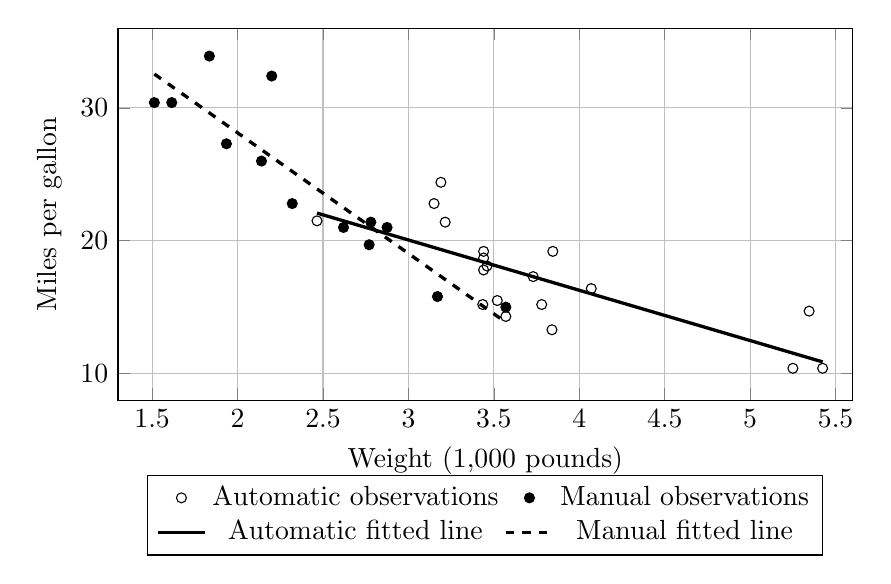
\begin{tikzpicture}
\begin{axis}[
    width=0.9\textwidth,
    height=0.52\textwidth,
    xlabel={Weight (1,000 pounds)},
    ylabel={Miles per gallon},
    xmin=1.3, xmax=5.6,
    ymin=8, ymax=36,
    legend style={at={(0.5,-0.20)},anchor=north,legend columns=2},
    grid=major
]
\addplot[only marks,mark=o,mark size=1.8pt] coordinates {
(3.215,21.4)
(3.440,18.7)
(3.460,18.1)
(3.570,14.3)
(3.190,24.4)
(3.150,22.8)
(3.440,19.2)
(3.440,17.8)
(4.070,16.4)
(3.730,17.3)
(3.780,15.2)
(5.250,10.4)
(5.424,10.4)
(5.345,14.7)
(2.465,21.5)
(3.520,15.5)
(3.435,15.2)
(3.840,13.3)
(3.845,19.2)
};
\addlegendentry{Automatic observations}

\addplot[only marks,mark=*,mark size=1.8pt] coordinates {
(2.620,21.0)
(2.875,21.0)
(2.320,22.8)
(2.200,32.4)
(1.615,30.4)
(1.835,33.9)
(1.935,27.3)
(2.140,26.0)
(1.513,30.4)
(3.170,15.8)
(2.770,19.7)
(3.570,15.0)
(2.780,21.4)
};
\addlegendentry{Manual observations}

\addplot[domain=2.465:5.424,samples=2,very thick] {31.416055 - 3.785908*x};
\addlegendentry{Automatic fitted line}

\addplot[domain=1.513:3.570,samples=2,very thick,dashed] {46.294478 - 9.084268*x};
\addlegendentry{Manual fitted line}
\end{axis}
\end{tikzpicture}
\caption{An interaction permits the fitted relationship between weight and fuel economy to have a different slope for automatic and manual cars. The lines are drawn only across each group's observed weight range.}
\label{fig:interaction_mtcars}
\end{figure}

The corresponding base-R graph is straightforward:

\begin{lstlisting}
fit_interaction <- lm(mpg ~ wt * am, data = mtcars)

plot(
  mtcars$wt,
  mtcars$mpg,
  pch = ifelse(mtcars$am == 0, 1, 19),
  xlab = "Weight (1,000 pounds)",
  ylab = "Miles per gallon",
  main = "Interaction: mpg ~ wt * am"
)

# Create separate x-grids over each group's observed support
auto_wt <- seq(
  min(mtcars$wt[mtcars$am == 0]),
  max(mtcars$wt[mtcars$am == 0]),
  length.out = 100
)

manual_wt <- seq(
  min(mtcars$wt[mtcars$am == 1]),
  max(mtcars$wt[mtcars$am == 1]),
  length.out = 100
)

auto_pred <- predict(
  fit_interaction,
  newdata = data.frame(wt = auto_wt, am = 0)
)

manual_pred <- predict(
  fit_interaction,
  newdata = data.frame(wt = manual_wt, am = 1)
)

lines(auto_wt, auto_pred, lwd = 3)
lines(manual_wt, manual_pred, lwd = 3, lty = 2)

legend(
  "topright",
  legend = c("Automatic", "Manual"),
  pch = c(1, 19),
  lty = c(1, 2),
  lwd = c(3, 3),
  bty = "n"
)
\end{lstlisting}

Notice that the plotted lines stop at the observed range for each group. That choice anticipates the next topic: extrapolation.

\section{Interaction Effects Depend on the Value of the Other Variable}

Once an interaction is present, there is generally no single coefficient that describes ``the effect of \(X\)'' everywhere in the fitted model.

For
\[
\widehat{Y}
=
\widehat{\beta}_0+
\widehat{\beta}_1X+
\widehat{\beta}_2Z+
\widehat{\beta}_3XZ,
\]
the fitted change in \(Y\) associated with a one-unit increase in \(X\), holding \(Z\) at a particular value, is
\[
\widehat{\beta}_1+
\widehat{\beta}_3Z.
\]

Thus the relationship between \(X\) and the fitted outcome depends on \(Z\). Likewise, the relationship between \(Z\) and the fitted outcome depends on \(X\).

For a binary \(Z\), this yields two group-specific slopes. For two continuous variables, the slope can vary continuously with the value of the interacting variable.

This is why interactions should be interpreted through predicted values or marginal comparisons rather than by reading each coefficient in isolation.

\section{Interpolation, Support, and Extrapolation}
\index{interpolation}\index{support}\index{extrapolation}

Suppose the observed \(X\)-values range from 2 to 10.

A prediction at \(X=6\) is an \emph{interpolation}: it lies within the region covered by the observed predictor values.

A prediction at \(X=15\) is an \emph{extrapolation}: it lies outside that region.

Why does the distinction matter?

Inside the observed range, the data constrain the fitted function. If a proposed curve behaves badly at \(X=6\), observations near \(X=6\) can expose that problem.

Outside the observed range, there are no outcomes available to discipline the shape of the fitted relationship. The regression simply extends the mathematical form that was estimated inside the data.

For a straight-line regression, it extends the line.

For a quadratic regression, it extends the parabola.

For a cubic regression, it extends the cubic polynomial.

The regression software can calculate all of these predictions perfectly. The problem is not computational. The problem is that the data may tell us very little about which extension is credible.

\section{Interpolation Is Not Automatically Safe}
\index{interpolation!risks}\index{support!gaps}\index{data gaps}

It is tempting to turn the interpolation--extrapolation distinction into a simple rule:

\begin{quote}
Interpolation is safe; extrapolation is dangerous.
\end{quote}

That rule is too simple. Interpolation is \emph{usually} better supported than extrapolation, but merely being between the smallest and largest observed values of a predictor does not guarantee that a prediction is well supported by the data.

Suppose the observed values of \(X\) fall into two clusters: many observations between 1 and 4, and many observations between 7 and 10, with almost nothing between 4 and 7. A prediction at \(X=5.5\) is technically inside the observed minimum and maximum. In the simplest one-dimensional sense it is therefore an interpolation. But there are no nearby observations telling us what the conditional expectation function actually does around \(X=5.5\).

The fitted model must bridge the gap. How it bridges the gap depends on functional-form assumptions.

\begin{center}
\fbox{
\parbox{0.88\textwidth}{
\centering
\textbf{Inside the min--max range does not necessarily mean well supported.}

\vspace{0.4em}

A prediction can be an interpolation and still depend heavily on assumptions if the training data are sparse or absent near the requested predictor values.
}
}
\end{center}

\subsection{A gap inside the observed range}

The following artificial example makes the problem visible. The data contain observations on both sides of a large gap, but none inside it.

\begin{lstlisting}
set.seed(26)

x_left  <- runif(35, min = 1, max = 4)
x_right <- runif(35, min = 7, max = 10)

x <- c(x_left, x_right)

y <- c(
  2 + 3 * x_left  + rnorm(35, mean = 0, sd = 0.5),
  28 - x_right + rnorm(35, mean = 0, sd = 0.5)
)

gap_data <- data.frame(x = x, y = y)

fit_linear <- lm(y ~ x, data = gap_data)
fit_quadratic <- lm(y ~ x + I(x^2), data = gap_data)

# Both models can produce a prediction at x = 5.5,
# even though there are no training observations nearby.
new_point <- data.frame(x = 5.5)

predict(fit_linear, newdata = new_point)
predict(fit_quadratic, newdata = new_point)
\end{lstlisting}

With this particular random seed, the straight-line model predicts approximately \(14.5\) at \(X=5.5\), while the quadratic model predicts approximately \(17.9\). Both numbers are produced without computational difficulty. Neither is directly checked by observations near \(5.5\), because there are none.

The point is not that the quadratic answer is correct and the linear answer is wrong. The point is that \emph{the data leave the behavior inside the gap underdetermined}. A straight line, a smooth curve, a threshold, or some other process could connect the two observed regions differently.

The gap can be displayed directly in base R:

\begin{lstlisting}
# Grid used to draw fitted functions
x_grid <- seq(1, 10, length.out = 300)
new_grid <- data.frame(x = x_grid)

linear_hat <- predict(
  fit_linear,
  newdata = new_grid
)

quadratic_hat <- predict(
  fit_quadratic,
  newdata = new_grid
)

plot(
  gap_data$x,
  gap_data$y,
  xlab = "X",
  ylab = "Y",
  main = "Interpolation Across a Gap in the Training Data",
  pch = 19
)

# Mark the unsupported interior region.
rect(
  xleft = 4,
  ybottom = par("usr")[3],
  xright = 7,
  ytop = par("usr")[4],
  density = 12,
  angle = 45,
  border = NA
)

# Redraw points so they remain visible after shading.
points(gap_data$x, gap_data$y, pch = 19)

lines(x_grid, linear_hat, lwd = 3)
lines(x_grid, quadratic_hat, lwd = 3, lty = 2)

abline(v = c(4, 7), lty = 3)

points(
  5.5,
  predict(fit_linear, newdata = data.frame(x = 5.5)),
  pch = 1,
  cex = 1.5,
  lwd = 2
)

points(
  5.5,
  predict(fit_quadratic, newdata = data.frame(x = 5.5)),
  pch = 2,
  cex = 1.5,
  lwd = 2
)

legend(
  "topleft",
  legend = c(
    "Linear fit",
    "Quadratic fit",
    "Gap with no training observations"
  ),
  lty = c(1, 2, NA),
  lwd = c(3, 3, NA),
  fill = c(NA, NA, "black"),
  density = c(0, 0, 35),
  angle = 45,
  border = c(NA, NA, "black"),
  bty = "n"
)
\end{lstlisting}

This example gives us a more precise way to talk about interpolation. A prediction may be \emph{inside the overall range} of \(X\) while still being far from the observations that trained the model. In such a region, the assumed functional form can do much more of the work than the word ``interpolation'' suggests.

\subsection{Sparse regions create the same problem more gradually}

A literal empty gap is an extreme case. The same issue arises gradually when observations are merely sparse. Imagine 1,000 observations near \(X=2\), another 1,000 near \(X=8\), and only two observations near \(X=5\). A prediction at \(X=5\) is not unsupported in an all-or-nothing sense, but it is much less empirically anchored than a prediction at \(X=2\) or \(X=8\).

This is one reason it is useful to look at the distribution of predictors rather than merely reporting their minimum and maximum. Scatterplots, histograms, rug marks, and counts in local neighborhoods can reveal whether a nominal interpolation is actually taking place in a data-rich region.

\subsection{With several predictors, the problem is more important}
\index{support!multidimensional}\index{interpolation!multidimensional}

In multiple regression, checking each predictor's range separately is not enough.

Suppose the training data contain:

\begin{itemize}
    \item people aged 20--30 with incomes between \$20,000 and \$50,000; and
    \item people aged 55--70 with incomes between \$100,000 and \$200,000.
\end{itemize}

Now ask for a prediction for a 22-year-old earning \$180,000. Age 22 is inside the observed age range. Income \$180,000 is inside the observed income range. Yet the \emph{combination} \((22,180{,}000)\) may be nowhere near any training observation.

A multiple regression can still calculate a prediction. Algebraically, nothing prevents it. Empirically, however, the prediction is relying on the model to combine predictor values in a region where the joint data provide little guidance.

This is why \emph{support} is a better concept than the one-dimensional min--max range. In several dimensions, support concerns the predictor combinations that are actually represented by observations.

The distinction becomes crucial for causal inference. A treated unit may have values of every covariate that individually fall within the control group's range while nevertheless having a combination of covariates unlike any control unit. Calling the required prediction ``interpolation'' merely because each variable is separately in range can therefore be misleading.

A useful hierarchy is:

\begin{enumerate}
    \item \textbf{Dense local support:} many training observations lie near the requested predictor value or combination. Prediction is relatively data-driven.
    \item \textbf{Sparse interpolation:} the requested value is inside the broad support or range, but relatively few observations lie nearby. Functional-form assumptions matter more.
    \item \textbf{Gap interpolation:} the requested value lies between observed regions but in a local hole with essentially no observations. The model must bridge the gap.
    \item \textbf{Extrapolation:} the requested value or predictor combination lies beyond the region represented by the training data. Functional-form assumptions can dominate.
\end{enumerate}

These categories are not perfectly sharp in every dataset. Their purpose is to replace the false binary idea that all interpolation is safe while all extrapolation is unsafe.

The practical question is always:

\begin{quote}
\textbf{How much nearby training information actually supports this prediction?}
\end{quote}

\section{Empirical Example: Old Faithful and Functional-Form Dependence}
\index{faithful data set@\texttt{faithful} data set}

The built-in R dataset \texttt{faithful} contains 272 observations on eruptions of the Old Faithful geyser. We will predict the waiting time until the next eruption from the duration of the current eruption.

The observed eruption durations range from about 1.6 to 5.1 minutes.

Fit three OLS models:

\begin{lstlisting}
fit_linear <- lm(waiting ~ eruptions, data = faithful)

fit_quadratic <- lm(
  waiting ~ eruptions + I(eruptions^2),
  data = faithful
)

fit_cubic <- lm(
  waiting ~ eruptions + I(eruptions^2) + I(eruptions^3),
  data = faithful
)

summary(fit_linear)$r.squared
summary(fit_quadratic)$r.squared
summary(fit_cubic)$r.squared
\end{lstlisting}

Their training-sample \(R^2\) values are approximately
\[
0.811,\qquad 0.821,\qquad 0.827.
\]

Within the observed data, all three models capture much of the relationship. The quadratic and cubic models improve training \(R^2\) only modestly relative to the straight line.

Now ask each model to predict a waiting time following a hypothetical seven-minute eruption:

\begin{lstlisting}
new_case <- data.frame(eruptions = 7)

predict(fit_linear, newdata = new_case)
predict(fit_quadratic, newdata = new_case)
predict(fit_cubic, newdata = new_case)
\end{lstlisting}

The predictions are dramatically different:
\[
\begin{array}{lcc}
\toprule
\text{Model} & \text{Predicted waiting time at 7 minutes} \\
\midrule
\text{Linear} & 108.6 \\
\text{Quadratic} & 86.1 \\
\text{Cubic} & 19.8 \\
\bottomrule
\end{array}
\]

Nothing happened to the data. We changed only the assumed functional form. Because seven minutes is well beyond the observed maximum of 5.1 minutes, the data provide no direct evidence about which mathematical extension is appropriate.

Figure~\ref{fig:faithful_extrapolation} makes the problem visible. The vertical line marks the maximum observed eruption duration. To the left of that line, the functions are disciplined by actual observations. To the right, they are extrapolations.

\begin{figure}[H]
\centering
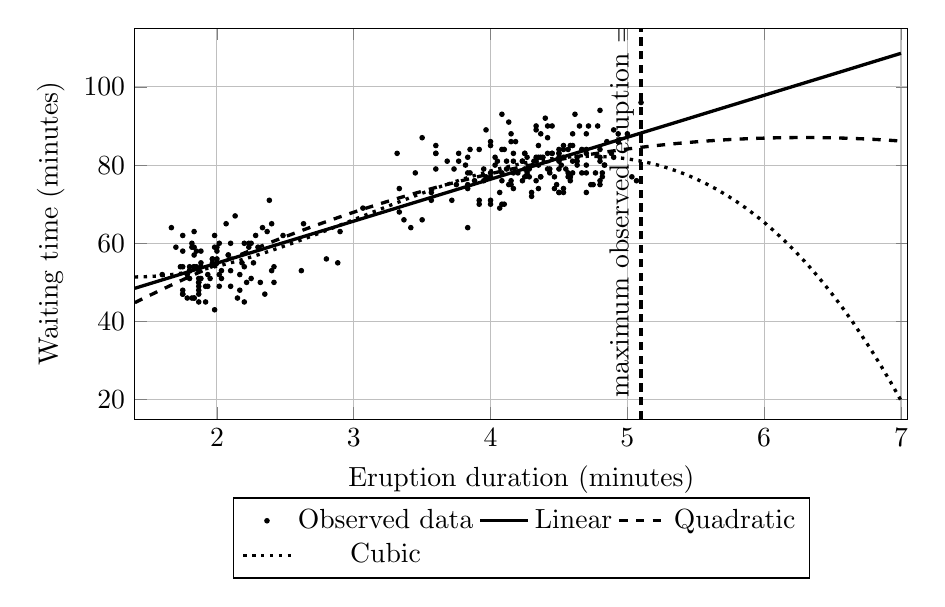
\begin{tikzpicture}
\begin{axis}[
    width=0.94\textwidth,
    height=0.54\textwidth,
    xlabel={Eruption duration (minutes)},
    ylabel={Waiting time (minutes)},
    xmin=1.4, xmax=7.05,
    ymin=15, ymax=115,
    legend style={at={(0.5,-0.20)},anchor=north,legend columns=3},
    grid=major
]
\addplot[only marks,mark=*,mark size=0.8pt] coordinates {
(3.600,79.0)
(1.800,54.0)
(3.333,74.0)
(2.283,62.0)
(4.533,85.0)
(2.883,55.0)
(4.700,88.0)
(3.600,85.0)
(1.950,51.0)
(4.350,85.0)
(1.833,54.0)
(3.917,84.0)
(4.200,78.0)
(1.750,47.0)
(4.700,83.0)
(2.167,52.0)
(1.750,62.0)
(4.800,84.0)
(1.600,52.0)
(4.250,79.0)
(1.800,51.0)
(1.750,47.0)
(3.450,78.0)
(3.067,69.0)
(4.533,74.0)
(3.600,83.0)
(1.967,55.0)
(4.083,76.0)
(3.850,78.0)
(4.433,79.0)
(4.300,73.0)
(4.467,77.0)
(3.367,66.0)
(4.033,80.0)
(3.833,74.0)
(2.017,52.0)
(1.867,48.0)
(4.833,80.0)
(1.833,59.0)
(4.783,90.0)
(4.350,80.0)
(1.883,58.0)
(4.567,84.0)
(1.750,58.0)
(4.533,73.0)
(3.317,83.0)
(3.833,64.0)
(2.100,53.0)
(4.633,82.0)
(2.000,59.0)
(4.800,75.0)
(4.716,90.0)
(1.833,54.0)
(4.833,80.0)
(1.733,54.0)
(4.883,83.0)
(3.717,71.0)
(1.667,64.0)
(4.567,77.0)
(4.317,81.0)
(2.233,59.0)
(4.500,84.0)
(1.750,48.0)
(4.800,82.0)
(1.817,60.0)
(4.400,92.0)
(4.167,78.0)
(4.700,78.0)
(2.067,65.0)
(4.700,73.0)
(4.033,82.0)
(1.967,56.0)
(4.500,79.0)
(4.000,71.0)
(1.983,62.0)
(5.067,76.0)
(2.017,60.0)
(4.567,78.0)
(3.883,76.0)
(3.600,83.0)
(4.133,75.0)
(4.333,82.0)
(4.100,70.0)
(2.633,65.0)
(4.067,73.0)
(4.933,88.0)
(3.950,76.0)
(4.517,80.0)
(2.167,48.0)
(4.000,86.0)
(2.200,60.0)
(4.333,90.0)
(1.867,50.0)
(4.817,78.0)
(1.833,63.0)
(4.300,72.0)
(4.667,84.0)
(3.750,75.0)
(1.867,51.0)
(4.900,82.0)
(2.483,62.0)
(4.367,88.0)
(2.100,49.0)
(4.500,83.0)
(4.050,81.0)
(1.867,47.0)
(4.700,84.0)
(1.783,52.0)
(4.850,86.0)
(3.683,81.0)
(4.733,75.0)
(2.300,59.0)
(4.900,89.0)
(4.417,79.0)
(1.700,59.0)
(4.633,81.0)
(2.317,50.0)
(4.600,85.0)
(1.817,59.0)
(4.417,87.0)
(2.617,53.0)
(4.067,69.0)
(4.250,77.0)
(1.967,56.0)
(4.600,88.0)
(3.767,81.0)
(1.917,45.0)
(4.500,82.0)
(2.267,55.0)
(4.650,90.0)
(1.867,45.0)
(4.167,83.0)
(2.800,56.0)
(4.333,89.0)
(1.833,46.0)
(4.383,82.0)
(1.883,51.0)
(4.933,86.0)
(2.033,53.0)
(3.733,79.0)
(4.233,81.0)
(2.233,60.0)
(4.533,82.0)
(4.817,77.0)
(4.333,76.0)
(1.983,59.0)
(4.633,80.0)
(2.017,49.0)
(5.100,96.0)
(1.800,53.0)
(5.033,77.0)
(4.000,77.0)
(2.400,65.0)
(4.600,81.0)
(3.567,71.0)
(4.000,70.0)
(4.500,81.0)
(4.083,93.0)
(1.800,53.0)
(3.967,89.0)
(2.200,45.0)
(4.150,86.0)
(2.000,58.0)
(3.833,78.0)
(3.500,66.0)
(4.583,76.0)
(2.367,63.0)
(5.000,88.0)
(1.933,52.0)
(4.617,93.0)
(1.917,49.0)
(2.083,57.0)
(4.583,77.0)
(3.333,68.0)
(4.167,81.0)
(4.333,81.0)
(4.500,73.0)
(2.417,50.0)
(4.000,85.0)
(4.167,74.0)
(1.883,55.0)
(4.583,77.0)
(4.250,83.0)
(3.767,83.0)
(2.033,51.0)
(4.433,78.0)
(4.083,84.0)
(1.833,46.0)
(4.417,83.0)
(2.183,55.0)
(4.800,81.0)
(1.833,57.0)
(4.800,76.0)
(4.100,84.0)
(3.966,77.0)
(4.233,81.0)
(3.500,87.0)
(4.366,77.0)
(2.250,51.0)
(4.667,78.0)
(2.100,60.0)
(4.350,82.0)
(4.133,91.0)
(1.867,53.0)
(4.600,78.0)
(1.783,46.0)
(4.367,77.0)
(3.850,84.0)
(1.933,49.0)
(4.500,83.0)
(2.383,71.0)
(4.700,80.0)
(1.867,49.0)
(3.833,75.0)
(3.417,64.0)
(4.233,76.0)
(2.400,53.0)
(4.800,94.0)
(2.000,55.0)
(4.150,76.0)
(1.867,50.0)
(4.267,82.0)
(1.750,54.0)
(4.483,75.0)
(4.000,78.0)
(4.117,79.0)
(4.083,78.0)
(4.267,78.0)
(3.917,70.0)
(4.550,79.0)
(4.083,70.0)
(2.417,54.0)
(4.183,86.0)
(2.217,50.0)
(4.450,90.0)
(1.883,54.0)
(1.850,54.0)
(4.283,77.0)
(3.950,79.0)
(2.333,64.0)
(4.150,75.0)
(2.350,47.0)
(4.933,86.0)
(2.900,63.0)
(4.583,85.0)
(3.833,82.0)
(2.083,57.0)
(4.367,82.0)
(2.133,67.0)
(4.350,74.0)
(2.200,54.0)
(4.450,83.0)
(3.567,73.0)
(4.500,73.0)
(4.150,88.0)
(3.817,80.0)
(3.917,71.0)
(4.450,83.0)
(2.000,56.0)
(4.283,79.0)
(4.767,78.0)
(4.533,84.0)
(1.850,58.0)
(4.250,83.0)
(1.983,43.0)
(2.250,60.0)
(4.750,75.0)
(4.117,81.0)
(2.150,46.0)
(4.417,90.0)
(1.817,46.0)
(4.467,74.0)
};
\addlegendentry{Observed data}

\addplot[very thick] coordinates {
(1.400,48.496)
(1.471,49.256)
(1.542,50.017)
(1.613,50.778)
(1.684,51.538)
(1.754,52.299)
(1.825,53.059)
(1.896,53.820)
(1.967,54.581)
(2.038,55.341)
(2.109,56.102)
(2.180,56.862)
(2.251,57.623)
(2.322,58.383)
(2.392,59.144)
(2.463,59.905)
(2.534,60.665)
(2.605,61.426)
(2.676,62.186)
(2.747,62.947)
(2.818,63.708)
(2.889,64.468)
(2.959,65.229)
(3.030,65.989)
(3.101,66.750)
(3.172,67.510)
(3.243,68.271)
(3.314,69.032)
(3.385,69.792)
(3.456,70.553)
(3.527,71.313)
(3.597,72.074)
(3.668,72.835)
(3.739,73.595)
(3.810,74.356)
(3.881,75.116)
(3.952,75.877)
(4.023,76.637)
(4.094,77.398)
(4.165,78.159)
(4.235,78.919)
(4.306,79.680)
(4.377,80.440)
(4.448,81.201)
(4.519,81.962)
(4.590,82.722)
(4.661,83.483)
(4.732,84.243)
(4.803,85.004)
(4.873,85.764)
(4.944,86.525)
(5.015,87.286)
(5.086,88.046)
(5.157,88.807)
(5.228,89.567)
(5.299,90.328)
(5.370,91.088)
(5.441,91.849)
(5.511,92.610)
(5.582,93.370)
(5.653,94.131)
(5.724,94.891)
(5.795,95.652)
(5.866,96.413)
(5.937,97.173)
(6.008,97.934)
(6.078,98.694)
(6.149,99.455)
(6.220,100.215)
(6.291,100.976)
(6.362,101.737)
(6.433,102.497)
(6.504,103.258)
(6.575,104.018)
(6.646,104.779)
(6.716,105.540)
(6.787,106.300)
(6.858,107.061)
(6.929,107.821)
(7.000,108.582)
};
\addlegendentry{Linear}

\addplot[very thick,dashed] coordinates {
(1.400,44.837)
(1.471,46.052)
(1.542,47.249)
(1.613,48.429)
(1.684,49.591)
(1.754,50.735)
(1.825,51.861)
(1.896,52.970)
(1.967,54.061)
(2.038,55.134)
(2.109,56.190)
(2.180,57.227)
(2.251,58.247)
(2.322,59.249)
(2.392,60.234)
(2.463,61.201)
(2.534,62.149)
(2.605,63.081)
(2.676,63.994)
(2.747,64.890)
(2.818,65.768)
(2.889,66.628)
(2.959,67.470)
(3.030,68.295)
(3.101,69.102)
(3.172,69.891)
(3.243,70.662)
(3.314,71.416)
(3.385,72.152)
(3.456,72.870)
(3.527,73.571)
(3.597,74.253)
(3.668,74.918)
(3.739,75.565)
(3.810,76.195)
(3.881,76.807)
(3.952,77.400)
(4.023,77.977)
(4.094,78.535)
(4.165,79.076)
(4.235,79.599)
(4.306,80.104)
(4.377,80.591)
(4.448,81.061)
(4.519,81.513)
(4.590,81.947)
(4.661,82.364)
(4.732,82.762)
(4.803,83.143)
(4.873,83.506)
(4.944,83.852)
(5.015,84.179)
(5.086,84.489)
(5.157,84.782)
(5.228,85.056)
(5.299,85.313)
(5.370,85.552)
(5.441,85.773)
(5.511,85.976)
(5.582,86.162)
(5.653,86.330)
(5.724,86.480)
(5.795,86.612)
(5.866,86.727)
(5.937,86.824)
(6.008,86.903)
(6.078,86.965)
(6.149,87.008)
(6.220,87.034)
(6.291,87.043)
(6.362,87.033)
(6.433,87.006)
(6.504,86.961)
(6.575,86.898)
(6.646,86.817)
(6.716,86.719)
(6.787,86.603)
(6.858,86.469)
(6.929,86.317)
(7.000,86.148)
};
\addlegendentry{Quadratic}

\addplot[very thick,dotted] coordinates {
(1.400,51.391)
(1.471,51.446)
(1.542,51.581)
(1.613,51.791)
(1.684,52.073)
(1.754,52.424)
(1.825,52.841)
(1.896,53.319)
(1.967,53.854)
(2.038,54.445)
(2.109,55.086)
(2.180,55.775)
(2.251,56.508)
(2.322,57.281)
(2.392,58.091)
(2.463,58.934)
(2.534,59.806)
(2.605,60.705)
(2.676,61.627)
(2.747,62.567)
(2.818,63.523)
(2.889,64.491)
(2.959,65.468)
(3.030,66.449)
(3.101,67.432)
(3.172,68.412)
(3.243,69.387)
(3.314,70.352)
(3.385,71.305)
(3.456,72.241)
(3.527,73.157)
(3.597,74.050)
(3.668,74.916)
(3.739,75.751)
(3.810,76.552)
(3.881,77.316)
(3.952,78.038)
(4.023,78.715)
(4.094,79.345)
(4.165,79.922)
(4.235,80.444)
(4.306,80.907)
(4.377,81.308)
(4.448,81.642)
(4.519,81.907)
(4.590,82.099)
(4.661,82.214)
(4.732,82.249)
(4.803,82.201)
(4.873,82.065)
(4.944,81.838)
(5.015,81.517)
(5.086,81.098)
(5.157,80.577)
(5.228,79.952)
(5.299,79.217)
(5.370,78.371)
(5.441,77.409)
(5.511,76.328)
(5.582,75.125)
(5.653,73.795)
(5.724,72.335)
(5.795,70.741)
(5.866,69.011)
(5.937,67.141)
(6.008,65.126)
(6.078,62.964)
(6.149,60.651)
(6.220,58.183)
(6.291,55.557)
(6.362,52.769)
(6.433,49.816)
(6.504,46.694)
(6.575,43.400)
(6.646,39.930)
(6.716,36.280)
(6.787,32.447)
(6.858,28.428)
(6.929,24.219)
(7.000,19.816)
};
\addlegendentry{Cubic}

\draw[very thick,densely dashed] (axis cs:5.1,15) -- (axis cs:5.1,115);
\node[anchor=south west,rotate=90] at (axis cs:5.12,18) {maximum observed eruption = 5.1};
\end{axis}
\end{tikzpicture}
\caption{Several functional forms describe the observed Old Faithful relationship reasonably well but make radically different predictions beyond the support of the data.}
\label{fig:faithful_extrapolation}
\end{figure}

The same visualization can be generated in base R:

\begin{lstlisting}
fit_linear <- lm(waiting ~ eruptions, data = faithful)
fit_quadratic <- lm(
  waiting ~ eruptions + I(eruptions^2),
  data = faithful
)
fit_cubic <- lm(
  waiting ~ eruptions + I(eruptions^2) + I(eruptions^3),
  data = faithful
)

x_grid <- seq(1.4, 7, length.out = 300)
new_grid <- data.frame(eruptions = x_grid)

plot(
  faithful$eruptions,
  faithful$waiting,
  xlim = c(1.4, 7),
  ylim = c(15, 115),
  xlab = "Eruption duration (minutes)",
  ylab = "Waiting time (minutes)",
  main = "Functional Form and Extrapolation"
)

lines(
  x_grid,
  predict(fit_linear, newdata = new_grid),
  lwd = 3,
  lty = 1
)

lines(
  x_grid,
  predict(fit_quadratic, newdata = new_grid),
  lwd = 3,
  lty = 2
)

lines(
  x_grid,
  predict(fit_cubic, newdata = new_grid),
  lwd = 3,
  lty = 3
)

abline(v = max(faithful$eruptions), lty = 2)

legend(
  "topleft",
  legend = c("Linear", "Quadratic", "Cubic"),
  lty = c(1, 2, 3),
  lwd = c(3, 3, 3),
  bty = "n"
)
\end{lstlisting}

This example illustrates an important principle:

\begin{quote}
\textbf{A model can interpolate well and still extrapolate disastrously.}
\end{quote}

Training fit does not tell us that the model's shape remains correct where no training data exist.

\section{Confidence and Prediction Intervals Do Not Solve Functional-Form Extrapolation}

Chapter~\ref{chap:intervals_multiple} distinguished uncertainty about the fitted conditional mean from uncertainty about a new observation. It may be tempting to think that a sufficiently wide confidence or prediction interval protects us automatically when we extrapolate.

Not necessarily.

Standard regression intervals are calculated \emph{conditional on the model form being used}. A confidence interval around a seven-minute prediction from the linear Old Faithful model quantifies uncertainty around the linear model's estimated extension. It does not ordinarily incorporate the possibility that a quadratic, cubic, threshold, or other functional form would extend the relationship differently.

Thus there are at least two conceptually different sources of uncertainty:

\begin{enumerate}
    \item \textbf{parameter uncertainty within a chosen model}, and
    \item \textbf{model-form uncertainty about which prediction function should be used at all}.\footnote{\emph{Model-form uncertainty} is uncertainty about the functional form or model class itself---for example, whether a relationship should be linear, quadratic, interaction-rich, or fit with a flexible smoother. Standard confidence and prediction intervals usually condition on the chosen model form; they do not automatically widen merely because another plausible specification would give a different answer.}
\end{enumerate}

Ordinary textbook confidence intervals primarily address the first. Extrapolation can make the second especially important.

\section{LOESS and Extrapolation}
\index{LOESS!extrapolation}

LOESS provides an instructive contrast. Because LOESS estimates relationships locally, it is naturally oriented toward interpolation. In R, the default LOESS prediction machinery commonly returns \texttt{NA} for predictor values outside the range covered by the fitted surface.

For example:

\begin{lstlisting}
fit_loess <- loess(waiting ~ eruptions, data = faithful)

predict(
  fit_loess,
  newdata = data.frame(eruptions = c(2, 4, 7))
)
\end{lstlisting}

The predictions at 2 and 4 minutes are within the observed range. A prediction at 7 minutes is outside the range and will ordinarily be unavailable under the default interpolating surface.

This is not a weakness. It is, in some ways, an honest reminder that flexible local methods do not automatically know what should happen where they have no neighboring data.

Parametric models such as straight lines and polynomials will usually extrapolate because their equations are defined outside the data. That mathematical ability should not be confused with empirical knowledge.

\section{Support in Multiple Regression}
\index{common support}\index{overlap}

With one predictor, support is easy to visualize: it is essentially the observed range of \(X\). With multiple predictors, support is multidimensional.

Suppose a dataset contains young people with low income and older people with high income, but almost no young people with very high income. A multiple regression can still generate a prediction for a 20-year-old with an extremely high income. The requested values may each be individually common, yet their \emph{combination} may be absent from the data.

This matters for interactions as well. In the \texttt{mtcars} data, automatic cars have weights ranging approximately from 2.47 to 5.42 thousand pounds, while manual cars range approximately from 1.51 to 3.57. The two groups overlap only over part of the weight range.

If we compare the fitted manual and automatic lines at a weight of 5, the automatic prediction is supported by observed automatic cars near that weight, but the manual prediction requires substantial extrapolation because no manual cars in the dataset are that heavy.

The regression formula will still return a number:

\begin{lstlisting}
fit_interaction <- lm(mpg ~ wt * am, data = mtcars)

predict(
  fit_interaction,
  newdata = data.frame(
    wt = c(5, 5),
    am = c(0, 1)
  )
)
\end{lstlisting}

But the two predictions are not equally supported by observed data.

This gives a useful rule for interpretation:

\begin{center}
\fbox{
\parbox{0.88\textwidth}{
\centering
Before interpreting a fitted comparison, ask not only \emph{``Can the regression calculate it?''} but also \emph{``Do the data contain observations near the predictor combinations needed for this comparison?''}
}
}
\end{center}

\section{How to Think About Functional Form in Practice}

There is no mechanical procedure that guarantees the correct functional form in real-world research. But several habits are useful.

\begin{enumerate}
    \item \textbf{Plot the data.} A scatterplot can reveal visible curvature, group differences, gaps in support, or unusual observations that a coefficient table hides.

    \item \textbf{Plot fitted values, not just coefficients.} Interactions and nonlinear terms are often far easier to understand as predicted lines or curves.

    \item \textbf{Ask what restrictions the formula imposes.} An additive group indicator imposes equal slopes. Omitting a squared term rules out quadratic curvature. A polynomial imposes a particular global shape.

    \item \textbf{Distinguish dense interpolation, sparse interpolation, gaps, and extrapolation.} Do not treat the observed minimum and maximum as a sufficient definition of support. Predictions near dense training data are more empirically anchored than predictions in sparse regions, interior gaps, unusual multivariable combinations, or beyond the observed support.

    \item \textbf{Compare plausible specifications.} If substantively reasonable models fit the observed data similarly but imply wildly different answers for the quantity of interest, that instability is important information.

    \item \textbf{Do not choose functional form solely to maximize training \(R^2\).} Adding polynomial terms or interactions cannot reduce training \(R^2\), but a more elaborate model can fit noise and behave badly outside the training sample.

    \item \textbf{Use subject-matter knowledge.} Known physical constraints, institutional rules, biological limits, or well-established mechanisms can tell us which mathematical forms are plausible and which are impossible.
\end{enumerate}

The goal is not necessarily to identify a uniquely correct equation in every application. It is to understand the assumptions built into the prediction machine and to know when the observed data strongly constrain the fitted relationship and when the assumed functional form has substantial influence on the result.

\section{Chapter Summary}

A regression specification determines the shapes of relationships that the model can learn. Straight-line models impose constant slopes. Polynomial and transformed predictors permit curvature while remaining linear in the coefficients.

Interactions relax additive restrictions. In a model with a binary group indicator and a continuous predictor, omitting the interaction forces the same slope in both groups. Adding \(X\times D\) allows group-specific slopes, and the interaction coefficient measures their difference.

Predictions also depend on where they are made. Interpolation is generally safer than extrapolation, but being between the minimum and maximum observed values does not guarantee strong empirical support. Data can contain sparse regions or literal gaps, and with multiple predictors a requested combination can be unsupported even when every predictor is individually within its observed range. Parametric equations bridge these gaps and continue mechanically beyond observed data, so functional-form assumptions can matter greatly both for weakly supported interpolation and for extrapolation. Confidence and prediction intervals do not automatically account for uncertainty about the chosen functional form.

The practical lesson is to inspect data support, visualize fitted relationships, interpret interactions through predictions, and treat extrapolation as a substantive modeling assumption rather than as an ordinary application of \texttt{predict()}.



\chapter{Regression, Overlap, Model Dependence, and Causal Inference}
\label{chap:causal_bridge}
\index{causal inference}\index{overlap}\index{model dependence}\index{randomized controlled trial}

This book is primarily about regression analysis, not about causal inference. But several of the most important ideas developed in the preceding chapters---prediction, functional form, interpolation, extrapolation, and support---become especially consequential when regression is used for causal questions.

The connection is simple to state. Causal inference requires us to learn about outcomes that were not observed. Regression is a prediction machine. It can therefore be used to construct predictions for those missing outcomes. The difficult part is deciding when those predictions are credible.

A useful organizing principle for this chapter is:

\begin{center}
\fbox{
\parbox{0.88\textwidth}{
\centering
\textbf{Good causal design reduces the amount of work we need the regression model to do.}
}}
\end{center}

When treated and control observations are genuinely comparable, causal conclusions can be anchored by observed comparisons. When they are not, the regression model must fill in more of the missing counterfactual information, and causal estimates become more dependent on functional-form assumptions.

\section{Counterfactuals Turn Causal Inference into a Prediction Problem}
\index{counterfactual}\index{potential outcome}

Suppose each unit has two potential outcomes:
\[
Y_i(1)
\]
under treatment and
\[
Y_i(0)
\]
under control. The individual causal effect is
\[
\tau_i=Y_i(1)-Y_i(0).
\]

For any one unit, however, we ordinarily observe only one of these two outcomes. If unit \(i\) receives treatment, we observe \(Y_i(1)\) but not \(Y_i(0)\). The missing outcome \(Y_i(0)\) is the counterfactual. If the unit receives control, the missing counterfactual is instead \(Y_i(1)\).

Regression can help because it can predict outcomes conditional on observed information. For a treated unit with pretreatment covariates \(X_i=x\), for example, we might try to estimate
\[
E[Y(0)\mid X=x]
\]
from untreated observations and use that fitted conditional expectation as a prediction of the missing untreated outcome.

This looks very much like ordinary regression prediction. But the causal use of the prediction creates an additional requirement: the observations used to build the prediction must provide credible information about what would have happened to the treated unit under the alternative condition.

\section{Confounding and the Need for Overlap}
\index{confounding}\index{common support}

Suppose treatment status \(D\) is related to a pretreatment variable \(X\), and \(X\) also predicts the outcome. Then simply comparing treated and control mean outcomes may mix together two things:

\begin{enumerate}
    \item differences caused by treatment; and
    \item differences associated with the different values of \(X\) found in the treated and control groups.
\end{enumerate}

In such a situation, \(X\) is a confounding variable for the treatment-outcome comparison, assuming it is causally prior to treatment and satisfies the relevant causal conditions.

Regression is often used to adjust for such variables. For example,
\[
Y_i=\beta_0+\tau D_i+\beta_1X_i+\varepsilon_i
\]
compares fitted treated and control outcomes while holding \(X\) fixed.

But the phrase ``holding \(X\) fixed'' hides an important empirical question:

\begin{quote}
Do we actually observe both treated and control units at similar values of \(X\)?
\end{quote}

If the answer is yes, there is \emph{overlap} or \emph{common support}. If the answer is no, the regression may still produce a treatment-control comparison, but that comparison has to be generated partly or entirely through extrapolation.

Consider a treated unit with \(X=12\). If the control group contains many units with \(X\) near 12, then estimating the untreated counterfactual is largely an interpolation problem. If the control observations end at \(X=8\), predicting the untreated outcome at \(X=12\) asks the model to extend the control outcome relationship beyond the data that identify it.

That is not merely an ordinary prediction inconvenience. It can determine the causal answer.

\begin{center}
\fbox{
\parbox{0.90\textwidth}{
\centering
\textbf{Strong overlap} \(\longrightarrow\) counterfactuals supported by observed comparisons \(\longrightarrow\) less functional-form dependence.

\vspace{0.5em}

\textbf{Poor overlap} \(\longrightarrow\) counterfactual extrapolation \(\longrightarrow\) greater model dependence.
}}
\end{center}

\section{Overlap Is Multidimensional}
\index{overlap!multidimensional}\index{support!multidimensional}

The support discussion from Chapter~\ref{chap:functional_form} becomes especially important here. With several confounders, checking one variable at a time is not enough.

Suppose the covariates are age, income, and education. Treated and control groups might each contain people aged 55, people with low incomes, and people with graduate education. Yet there may be almost no control observations who are simultaneously 55, low-income, and graduate educated.

Every predictor is individually ``in range,'' while the relevant combination lies in a sparse or unsupported region of the joint covariate space.

A regression can still calculate a predicted counterfactual there. Standard software ordinarily does not flag that the requested comparison is weakly supported by the observed data; it simply evaluates the fitted equation at the requested predictor values.

For causal work, therefore, overlap should be thought of as overlap on the \emph{joint set of confounding variables}, not merely overlap in a collection of one-dimensional ranges.

\section{Model Dependence: When the Regression Specification Determines the Causal Answer}
\index{model dependence}\index{functional form!causal inference}

A causal estimate is \emph{model dependent} when reasonable changes in the statistical specification produce meaningfully different causal conclusions because the observed data do not tightly determine the required counterfactual predictions.

The following deliberately simple example makes the point visible. Suppose the untreated conditional outcome is curved:
\[
Y(0)=5+X+0.4X^2+\varepsilon,
\]
and treatment adds a constant effect of 6:
\[
Y(1)=Y(0)+6.
\]

Now imagine an observational dataset in which controls occur for \(X=0,1,\ldots,8\), while treated units occur for \(X=5,6,\ldots,16\). There is some overlap---from \(X=5\) through \(X=8\)---but much of each group's support is different.

The following base-R code constructs such a dataset:

\begin{lstlisting}
# Construct an observational dataset with limited overlap
x_control <- rep(0:8, each = 3)
x_treated <- rep(5:16, each = 3)

noise_control <- rep(c(-1, 0, 1), times = 9)
noise_treated <- rep(c(-1, 0, 1), times = 12)

Y0_control <- 5 + x_control + 0.4 * x_control^2 + noise_control
Y0_treated <- 5 + x_treated + 0.4 * x_treated^2 + noise_treated

D <- c(rep(0, length(x_control)),
       rep(1, length(x_treated)))

x <- c(x_control, x_treated)

Y <- c(Y0_control,
       Y0_treated + 6)

causal_dat <- data.frame(Y, D, x)
\end{lstlisting}

Now fit two regression adjustments. The first incorrectly forces the outcome relationship with \(X\) to be linear. The second permits the quadratic relationship that generated the data:

\begin{lstlisting}
fit_linear_adjustment <- lm(
  Y ~ D + x,
  data = causal_dat
)

fit_quadratic_adjustment <- lm(
  Y ~ D + x + I(x^2),
  data = causal_dat
)

coef(fit_linear_adjustment)["D"]
coef(fit_quadratic_adjustment)["D"]
\end{lstlisting}

The true treatment effect in this constructed example is 6. Yet using all observations, the misspecified linear adjustment estimates a treatment coefficient of only about 1.19, while the correctly specified quadratic regression returns 6.

Nothing went wrong with OLS as an optimization algorithm. The linear regression found the best-fitting plane available within its restricted model class. The problem is causal: because treatment status and \(X\) occupy substantially different regions, the fitted functional form is being asked to determine counterfactual comparisons where direct treated-control evidence is weak or absent.

\section{Restricting Attention to Overlap Reduces Model Dependence}
\index{trimming}\index{common support!restriction}

Now restrict the same data to the region where both treated and control observations actually occur:
\[
5\leq X\leq 8.
\]

\begin{lstlisting}
overlap_dat <- causal_dat[
  causal_dat$x >= 5 & causal_dat$x <= 8,
]

fit_linear_overlap <- lm(
  Y ~ D + x,
  data = overlap_dat
)

fit_quadratic_overlap <- lm(
  Y ~ D + x + I(x^2),
  data = overlap_dat
)

coef(fit_linear_overlap)["D"]
coef(fit_quadratic_overlap)["D"]
\end{lstlisting}

In this constructed example, both specifications now return the true treatment difference of 6. Why? Within the overlap region, treated and control observations occur at the same \(X\)-values. The treatment comparison is anchored by direct comparisons rather than by extending one group's fitted outcome function into regions occupied only by the other group.

This is an unusually tidy constructed example, so real data will rarely behave this perfectly. The principle, however, is general. Restricting attention to regions with genuine overlap often decreases the extent to which a causal estimate is driven by functional-form assumptions.

The tradeoff is equally important: trimming away unsupported observations changes the population about which we can make a causal statement. Better-supported inference for a narrower population can be preferable to a more ambitious estimate whose counterfactuals depend heavily on extrapolation.

\subsection{Visualizing the support problem in base R}

The following plot makes the overlap structure visible:

\begin{lstlisting}
plot(
  causal_dat$x,
  causal_dat$Y,
  pch = ifelse(causal_dat$D == 1, 19, 1),
  xlab = "Confounder X",
  ylab = "Observed outcome Y",
  main = "Limited Overlap in an Observational Study"
)

abline(v = 5, lty = 3)
abline(v = 8, lty = 3)

legend(
  "topleft",
  legend = c("Control", "Treated", "Overlap: X = 5 to 8"),
  pch = c(1, 19, NA),
  lty = c(NA, NA, 3),
  bty = "n"
)
\end{lstlisting}

The important feature is not simply that the two groups have different average \(X\). It is that large portions of their covariate support do not overlap. A regression can compare treated and control predictions there, but those comparisons necessarily lean more heavily on model structure.

\section{Why Randomized Experiments Are Different}
\index{randomization}\index{randomized controlled trial}\index{RCT|see{randomized controlled trial}}

Randomized controlled trials are unusually reliable for causal inference because treatment assignment is created by a known random mechanism rather than by the ordinary processes that generate treatment selection.

Under random assignment,
\[
D \perp \{Y(0),Y(1),X\}
\]
in the assignment mechanism. In words, treatment assignment is independent of pretreatment characteristics and potential outcomes by design, apart from chance imbalance in the realized sample.

Consequently, the untreated group provides a direct estimate of what would, on average, have happened to the treated group under control, and the treated group provides a direct estimate of what would have happened under treatment.

For a simple two-arm randomized experiment, the fundamental estimator can therefore be nothing more complicated than
\[
\widehat{\tau}
=
\overline{Y}_{T}-\overline{Y}_{C}.
\]

As Chapter 2 showed, this is exactly the OLS coefficient from a regression containing only a binary treatment indicator:
\[
Y_i=\beta_0+\tau D_i+\varepsilon_i.
\]

The strength of the experiment does not come from the sophistication of this regression. It comes from the research design that makes the treated-control comparison credible.

Randomization also tends to produce overlap in pretreatment covariates because treated and control units are sampled, through the assignment mechanism, from the same underlying pool of study units. In a finite sample, especially a small one, exact balance is not guaranteed. But systematic separation of the sort produced by strong confounding is not built into the assignment process.

This is why a useful contrast is:

\begin{center}
\fbox{
\parbox{0.90\textwidth}{
\centering
\textbf{In a well-designed RCT, the design does most of the causal identification work and regression can play a supporting role.}

\vspace{0.5em}

\textbf{In a poorly overlapping observational study, regression may be asked to do work that the design has not made credible.}
}}
\end{center}

\section{Regression Adjustment in an RCT Is Not the Same as Regression Repair}
\index{regression adjustment}\index{precision}

Regression can still be useful in a randomized experiment. Pretreatment covariates can be added to improve precision, account for chance imbalance, or estimate heterogeneous treatment effects.

For example,
\[
Y_i=\beta_0+\tau D_i+\beta_1X_i+\varepsilon_i
\]
may predict outcomes more accurately than a treatment-only regression if \(X\) is strongly predictive of \(Y\).

But conceptually this is different from using regression in an observational study to remove systematic treatment-selection bias. In the RCT, randomization supplies the basic causal identification. The regression is not ordinarily being asked to invent the missing untreated outcomes for a treated population that lives in a completely different covariate region.

This distinction is worth remembering:

\begin{quote}
Regression adjustment after good design is not the same thing as asking regression to compensate for bad design.
\end{quote}

\section{Observational Design Can Reduce the Burden on the Outcome Model}
\index{matching}\index{subclassification}\index{trimming}\index{weighting}\index{propensity score}

Observational studies do not have random assignment, but analysts can often improve the design before fitting an outcome regression.

Methods such as matching, subclassification, trimming, and weighting---often implemented with the help of a propensity score---can be used to make treated and control groups more comparable on measured pretreatment confounders or to focus the analysis on regions with adequate overlap.\footnote{Briefly: \emph{matching} pairs each treated unit with one or more control units that have similar covariate values; \emph{subclassification} divides the sample into strata of similar covariate values and compares treated and control units within strata; \emph{trimming} discards units in regions where the other group has no comparable observations; and \emph{weighting} reweights observations so the treated and control covariate distributions more closely resemble one another. A \emph{propensity score} is the probability of receiving treatment given the measured covariates, and estimated propensity scores are often used to implement these methods. Each operates on the design---which units are compared---rather than on the outcome model.}

These methods do not make observational data equivalent to an RCT. They cannot eliminate confounding from important unmeasured variables merely by balancing measured ones. But they can make an important contribution: they can reduce the distance over which the outcome model must extrapolate.

This provides a useful way to think about the division of labor between design and modeling:

\begin{enumerate}
    \item \textbf{Design asks whether the comparison is supported.} Are there comparable treated and control observations? Which units belong to a region of common support?
    \item \textbf{Regression models outcomes within that comparison.} Given the supported data, what conditional prediction rule describes \(Y\)?
\end{enumerate}

When the design succeeds in creating strong comparability, several reasonable regression specifications should often tell broadly similar causal stories. When small changes in functional form produce radically different estimated effects, that sensitivity can be a warning that the data are asking the model to do too much.

\section{The Main Connection to Regression Analysis}

The point of this chapter is not that every regression should be interpreted causally. Most should not be unless the research design and assumptions justify doing so.

Rather, causal inference sharpens several lessons about regression that are already important for prediction:

\begin{itemize}
    \item A regression prediction is more trustworthy when it is supported by relevant training observations.
    \item Being inside each predictor's marginal range does not guarantee support in the joint predictor space.
    \item Functional-form choices matter more when predictions move away from observed data.
    \item Interpolation is generally less model dependent than extrapolation, but sparse interpolation can still be fragile.
    \item Software will produce a fitted value even when the requested comparison is poorly supported.
    \item Better research design reduces reliance on the regression model's unverifiable functional-form assumptions.
\end{itemize}

For causal inference, these points can be summarized in one sentence:

\begin{center}
\fbox{
\parbox{0.88\textwidth}{
\centering
\textbf{The farther a counterfactual prediction moves from an observed treated-control comparison toward unsupported extrapolation, the more the causal conclusion depends on the model rather than on the design.}
}}
\end{center}

This is one reason randomized experiments remain such an important benchmark. They are powerful not because they eliminate the need for statistical analysis, but because they arrange the data so that the central causal comparison is credible before a complicated regression model is ever fit.



\chapter{Regression Analysis: The Most Important Ideas}
\label{chap:summary}
\index{regression!conceptual summary}

Regression is best understood as a \emph{prediction machine}. Its basic task is to use information about predictors, conventionally called \(X\), to generate a prediction for an outcome \(Y\). For mean regression, the central target is the conditional expectation function
\[
E[Y\mid X=x],
\]
which asks what value of \(Y\) we should expect, on average, among units with particular values of \(X\).

The familiar straight-line model is only one version of this idea. Ordinary least squares can include transformations, polynomials, indicator variables, and interactions. Other likelihood-based regressions are designed for different dependent variables: logistic regression for binary outcomes, Poisson or negative binomial regression for counts, and other generalized models for other outcome types. LOESS estimates a flexible conditional mean locally rather than imposing one global parametric equation.

Every fitted regression optimizes an objective. OLS minimizes the sum of squared residuals, and therefore minimizes training-sample mean squared error within the class of prediction functions specified by the analyst. Logistic regression maximizes a Bernoulli likelihood, equivalently minimizing log loss. This optimization remains true even when the statistical model is misspecified. What misspecification threatens is not the fact that the fitting criterion was optimized, but the interpretation of the fitted model and the validity of conventional inferential guarantees.\footnote{By \emph{conventional inferential guarantees}, we mean the repeated-sampling properties claimed by standard model-based procedures. For example, under the assumptions used to derive the procedure, a nominal 95\% confidence interval should contain its target about 95\% of the time across repeated samples, and a test conducted at the 5\% level should reject a true null hypothesis about 5\% of the time. These guarantees apply to quantities such as standard errors, \(p\)-values, and confidence intervals; if the assumptions supporting the conventional formulas are materially wrong, the nominal coverage or error rates need not hold, even though the regression algorithm still optimizes its specified fitting criterion.}

Regression coefficients are instructions for how the prediction changes. With a single binary predictor, OLS produces a particularly simple result: the intercept is the mean outcome for the group coded zero, and the coefficient on the binary predictor is the difference in mean outcomes between the group coded one and the group coded zero. More generally, the fitted coefficients in an \texttt{lm()} object are exactly the numbers R uses when \texttt{predict()} constructs fitted values for either the original training observations or new cases.

In multiple regression, a coefficient is interpreted conditional on the other included predictors. In an additive model, the coefficient on \(X\) tells us how the fitted prediction changes when \(X\) increases by one unit while the other predictors are kept at fixed values. This is a statement about the fitted prediction function; it is not automatically a causal statement. Whether a regression coefficient can be interpreted causally requires a research design or assumptions that justify the relevant counterfactual comparison.

Interactions change coefficient interpretations. If a continuous predictor \(X\) and a binary group indicator \(D\) enter only additively, the model imposes the same slope on \(X\) in both groups. Adding \(X\times D\) allows the slopes to differ. With an interaction present, there is often no single universal ``effect of \(X\)'' in the fitted model: the fitted relationship between \(X\) and \(Y\) depends on the value of the interacting variable.

Prediction accuracy can be measured by mean squared error. In OLS with an intercept, the natural zero-predictor benchmark predicts the same number---the sample mean of \(Y\)---for every observation. \(R^2\) measures the fraction of that mean-only model's squared prediction error that disappears after predictors are introduced:
\[
R^2
=
1-
\frac{\text{MSE of fitted model}}
{\text{MSE of mean-only model}}.
\]
An \(R^2\) of zero means the fitted predictors do no better in-sample than predicting the mean for everyone. An \(R^2\) of one means every training observation is predicted perfectly. Adding predictors cannot lower ordinary training-sample \(R^2\), because OLS can always set the new coefficients to zero and reproduce the old fit. This is one reason a larger training \(R^2\) is not by itself evidence of a better model for new data.

Regression inference introduces several different uncertainty questions that must be named carefully. A confidence interval for a \emph{coefficient} describes uncertainty about a parameter such as \(\beta_1\). A confidence interval for a \emph{predicted conditional mean} describes uncertainty about where the regression line or regression surface lies at specified predictor values. A \emph{prediction interval} describes where a new individual outcome might lie. The last interval is ordinarily wider because it must include both uncertainty about the conditional mean and individual outcome variation around that mean.

The phrase ``confidence interval'' is therefore ambiguous. Students and analysts should specify the target: confidence interval for the slope coefficient, confidence interval for the fitted mean at \(X=x\), or prediction interval for a new observation at \(X=x\).

Likewise, a p-value has a specific inferential meaning. Under a stated null hypothesis and the assumptions used by the test, it measures how unusual the observed test statistic, or something more extreme, would be if the null were true. It is not the probability that the null hypothesis is true. A tiny p-value also does not necessarily imply a tight confidence interval: statistical significance depends partly on the estimate's scale and its distance from the null, whereas interval width depends on uncertainty measured in the units of the coefficient.

Confidence intervals and p-values achieve their nominal repeated-sampling properties only under the assumptions required by the inferential procedure. In textbook OLS, those assumptions concern the conditional mean specification and the error process; exact small-sample t procedures additionally invoke normality. Robust procedures can protect against some forms of misspecification, but no command can make inferential validity assumption-free. In most observational social-science problems, analysts do not know the true data-generating equation. Proper specification is therefore something to investigate and defend, not something to assume merely because software returned standard errors.

Functional form deserves the same caution. A linear model, quadratic model, cubic model, and flexible smoother can agree reasonably well where observations are plentiful and diverge where the data provide little guidance. Interpolation is generally safer than extrapolation, but ``inside the observed range'' is not synonymous with ``well supported.'' Interior gaps, sparse regions, and unusual combinations of multiple predictors can make an interpolation heavily dependent on modeling assumptions. Extrapolation goes further by extending the assumed shape beyond the region represented by the data. As nearby empirical support weakens, the functional form does more of the work. Conventional confidence or prediction intervals are usually conditional on the selected functional form and therefore do not automatically capture this model-form uncertainty.

Finally, regression connects to causal inference because causal questions require predictions of missing potential outcomes. Those counterfactual predictions are most credible when treated and control units overlap on relevant pretreatment confounders, so the comparison is anchored by observed data rather than by functional-form extrapolation. Poor overlap increases model dependence: different reasonable specifications can imply different counterfactuals. Randomized experiments are powerful precisely because the assignment design makes treated and control groups comparable in expectation, allowing the basic causal contrast to be identified with little dependence on an outcome-regression specification. Regression can still improve precision, but good design reduces the causal work the model must do.

The overall discipline of regression analysis is therefore to keep several questions separate: What is the prediction target? What loss function is being optimized? What functional form has been imposed? Where does the requested prediction lie relative to the training data? What kind of uncertainty interval is being reported? Which assumptions justify its coverage? And, if a causal interpretation is desired, what design or assumptions make the counterfactual prediction credible? Keeping those questions distinct prevents many of the most common conceptual mistakes in regression analysis.



\appendix
\chapter{Glossary}
\label{app:glossary}

\begin{description}[style=nextline,leftmargin=0pt,labelindent=0pt,font=\bfseries]
\item[Additive model] A regression in which predictor contributions enter as separate added terms, without interactions. With a group indicator and a continuous predictor, an additive model imposes the same continuous-predictor slope across groups.\index{additive model}

\item[Coefficient] An estimated parameter that determines how a fitted regression prediction changes as a predictor changes, given the model's functional form and the values of other included predictors.\index{regression coefficient}

\item[Common support / overlap] The region of joint predictor or confounder space in which the groups or conditions being compared have observed data. Strong overlap anchors comparisons in observed data; poor overlap forces greater reliance on extrapolation and functional-form assumptions.\index{common support}\index{overlap}

\item[Conditional expectation function (CEF)] The function \(E[Y\mid X=x]\), giving the expected value of an outcome conditional on specified predictor values.\index{conditional expectation function}

\item[Confounder] A pretreatment variable related to both treatment assignment and the outcome in a way that can distort an untreated-versus-treated comparison if it is not appropriately handled. Whether a variable is a confounder is a causal question, not something determined by a regression table alone.\index{confounder}\index{confounding}

\item[Confidence interval for a coefficient] An interval intended, under the assumptions of the inferential procedure, to have stated repeated-sampling coverage for a regression coefficient such as \(\beta_1\).\index{confidence interval!coefficient}

\item[Confidence interval for a predicted mean] An interval describing uncertainty about the conditional mean \(E[Y\mid X=x]\), or equivalently about where the fitted regression line or surface lies at specified predictor values.\index{confidence interval!predicted mean}

\item[Counterfactual] A potential outcome that was not observed because the unit experienced a different treatment or condition. Causal inference requires learning about such missing potential outcomes.\index{counterfactual}

\item[Extrapolation] Prediction at predictor values or combinations lying outside the support of the training data. Such predictions can be highly sensitive to functional-form assumptions.\index{extrapolation}

\item[Fitted value] The model's point prediction \(\widehat{Y}_i\) for an observation's outcome.\index{fitted value}

\item[Functional form] The mathematical shape permitted by a regression specification, such as straight-line, polynomial, logarithmic, or interaction-based relationships.\index{functional form}

\item[Interaction] A model term, such as \(X\times Z\), that allows the fitted relationship between one predictor and the outcome to depend on the value of another predictor.\index{interaction}

\item[Interpolation] Prediction at a predictor value lying between observed regions or within the broad range of the training data. Interpolation is generally safer than extrapolation, but it can still be weakly supported when observations are sparse, when there is an interior gap, or when a multivariable predictor combination has little or no nearby data.\index{interpolation}

\item[LOESS] A flexible local regression smoother that estimates the conditional mean using nearby observations rather than one global parametric equation.\index{LOESS}

\item[Loss function] A rule for scoring prediction errors. A fitting algorithm chooses model parameters to minimize a loss or, equivalently in many settings, maximize a likelihood.\index{loss function}

\item[Matching] A design method that pairs treated units with control units having similar pretreatment covariate values, so that comparisons are made between similar units rather than through model-based extrapolation.\index{matching}

\item[Mean-only model] An intercept-only OLS model that predicts the sample mean of \(Y\) for every observation. It provides the benchmark used in the usual definition of \(R^2\).\index{mean-only model}

\item[Mean squared error (MSE)] The average squared difference between observed outcomes and predicted outcomes.\index{mean squared error}

\item[Model dependence] Sensitivity of an estimated quantity to reasonable modeling choices such as functional form, interactions, or extrapolation rules. In causal inference, model dependence is often greatest where treated and control observations have poor overlap.\index{model dependence}

\item[Model misspecification] A mismatch between the statistical model's assumed structure and the actual data-generating process. Different inferential procedures are robust to different kinds of misspecification.\index{model misspecification}

\item[Multiple regression] A regression containing more than one predictor. Coefficients describe changes in the fitted prediction conditional on the other included predictors.\index{multiple regression}

\item[Ordinary least squares (OLS)] The regression fitting method that chooses coefficients to minimize the sum of squared residuals in the training sample.\index{ordinary least squares}\index{OLS}

\item[p-value] Under a specified null hypothesis and testing assumptions, the probability of obtaining a test statistic at least as extreme as the observed one if the null were true. It is not the probability that the null is true.\index{p-value}

\item[Potential outcome] The outcome a unit would experience under a particular treatment or condition. Only one potential outcome is ordinarily observed for a unit, leaving the alternatives counterfactual.\index{potential outcome}

\item[Prediction interval] An interval intended to describe where a new individual outcome may lie at specified predictor values. It is ordinarily wider than the confidence interval for the corresponding conditional mean.\index{prediction interval}

\item[Prediction machine] A useful conceptual description of regression: a rule that accepts predictor values as inputs and generates predictions for an outcome.\index{prediction machine}

\item[\(R^2\)] The fraction of the mean-only model's in-sample squared prediction error eliminated by the fitted OLS model. With an intercept, it ranges from 0 to 1 in ordinary applications.\index{R-squared@$R^2$}

\item[Randomized controlled trial (RCT)] An experiment in which treatment is assigned by a known random mechanism. Randomization makes treatment independent of pretreatment characteristics and potential outcomes in the assignment mechanism, providing a design-based foundation for causal comparison.\index{randomized controlled trial}

\item[Residual] The difference between an observed outcome and its fitted value, \(e_i=Y_i-\widehat{Y}_i\).\index{residual}

\item[Subclassification] A design method that divides the sample into strata (subclasses) of similar covariate values and compares treated and control units within each stratum before aggregating.\index{subclassification}

\item[Support] The region of predictor values or predictor combinations represented in the data. Support is local and, with multiple predictors, multidimensional; checking only each variable's minimum and maximum can conceal sparse or unsupported combinations.\index{support}

\item[Test set] Data not used to fit the model, used to assess how well the fitted prediction rule generalizes to new observations.\index{test set}

\item[Training set] The observations used to fit a model. Performance on the training set can be optimistic relative to performance on new data.\index{training set}

\item[Trimming] Restricting an analysis to the region of common support by discarding units whose covariate values have no counterparts in the comparison group.\index{trimming}

\item[Weighting] Reweighting observations so that the covariate distributions of treated and control groups become more comparable, reducing the adjustment burden placed on the outcome model.\index{weighting}
\end{description}

\cleardoublepage
\phantomsection
\addcontentsline{toc}{chapter}{Index}
{\small\printindex}

\end{document}
